\documentclass[aps,prd,reprint,nofootinbib,superscriptaddress]{revtex4-2}

\usepackage{graphicx}
\usepackage{hyperref}
\usepackage{amsmath, amssymb, amsfonts}
\usepackage{booktabs}
\usepackage{siunitx}
\usepackage{braket}

% Auto-generated by update_counts.py — 2026-10-14T09:43:30.211762
% Do not edit manually. Run: uv run python scripts/update_counts.py
\newcommand{\leantoolchain}{4.32.0}
\newcommand{\mathlibrev}{81a5d257}
\newcommand{\physlibrev}{c4843367}
\newcommand{\totaltheorems}{26353}
\newcommand{\substantivetheorems}{26327}
\newcommand{\placeholdertheorems}{26}
\newcommand{\kernelsubstantivetheorems}{26258}
\newcommand{\trackedvacuitydebt}{69}
\newcommand{\axiomcount}{0}
\newcommand{\sorrycount}{0}
\newcommand{\sorrypercent}{0.0}
\newcommand{\leanmodules}{2101}
\newcommand{\leandefinitions}{14045}
\newcommand{\pythonmodules}{138}
\newcommand{\testfiles}{214}
\newcommand{\totaltests}{7673}
\newcommand{\figurecount}{170}
\newcommand{\notebookcount}{91}
\newcommand{\papercount}{42}
\newcommand{\aristotleproved}{313}
\newcommand{\aristotleruns}{40}
% --- D11 bundle substrate summary (source-level, stated rule) ---
\newcommand{\dxiModules}{22}
\newcommand{\dxiLines}{6267}
\newcommand{\dxiTheorems}{403}
\newcommand{\dxiDefs}{82}
\newcommand{\dxiDepsTheorems}{409}
% --- Paper 18 / Phase 5t per-section counts (FermiHubbardDimer.lean) ---
\newcommand{\fhdTotal}{130}
\newcommand{\fhdWaveTwo}{13}
\newcommand{\fhdWaveThree}{6}
\newcommand{\fhdWaveFour}{19}
\newcommand{\fhdWaveFive}{20}
\newcommand{\fhdWaveSixABC}{35}
\newcommand{\fhdWaveSixExtra}{13}
\newcommand{\fhdWaveSeven}{17}
\newcommand{\fhdWaveEight}{7}
% --- Paper 26 / 27 per-module counts (BH entropy + four laws) ---
\newcommand{\bhEntropyTotal}{32}
\newcommand{\bhThermoTotal}{20}
% --- Phase 6 per-module + pytest counts (paper32 / paper34-38 / note_rt_ch_bounds) ---
\newcommand{\strongCpDeThms}{8}
\newcommand{\strongCpDeTests}{14}
\newcommand{\epThms}{24}
\newcommand{\epTests}{38}
\newcommand{\qecHolographyThms}{10}
\newcommand{\qecHolographyTests}{30}
\newcommand{\centerSymmThms}{18}
\newcommand{\centerSymmTests}{28}
\newcommand{\chiralSsbThms}{10}
\newcommand{\chiralSsbTests}{14}
\newcommand{\cflThms}{12}
\newcommand{\cflTests}{17}
\newcommand{\rtChThms}{7}
\newcommand{\rtChTests}{29}
\newcommand{\heatKernelThms}{20}
\newcommand{\heatKernelTests}{39}
\newcommand{\higherCurvatureThms}{13}
\newcommand{\higherCurvatureTests}{42}
\newcommand{\diffInvarianceThms}{13}
\newcommand{\diffInvarianceTests}{36}
\newcommand{\nonlinearEFEThms}{13}
\newcommand{\nonlinearEFETests}{40}
\newcommand{\microscopicCoefficientMatchThms}{12}
\newcommand{\microscopicCoefficientMatchTests}{42}
\newcommand{\einsteinCartanExtensionThms}{12}
\newcommand{\einsteinCartanExtensionTests}{41}
\newcommand{\bbnThms}{14}
\newcommand{\bbnTests}{16}
% --- Phase 6f/6g classical-GR per-module + wave totals (I1 §11–§13) ---
\newcommand{\curvatureThms}{14}
\newcommand{\einsteinTensorThms}{9}
\newcommand{\energyConditionsThms}{8}
\newcommand{\exactSolutionsThms}{16}
\newcommand{\admFormalismThms}{10}
\newcommand{\tetradFormalismThms}{5}
\newcommand{\phaseSixfWonesixTotal}{62}
\newcommand{\phaseSixfWsevenTotal}{13}
\newcommand{\riemannCoordinateThms}{8}
\newcommand{\riemannDifferentialBianchiThms}{8}
\newcommand{\bundleRiemannAuxThms}{6}
\newcommand{\bundleRiemannThms}{7}
\newcommand{\leviCivitaThms}{7}
\newcommand{\phaseSixfWeightTotal}{36}
\newcommand{\riccatiComparisonThms}{11}
\newcommand{\mazurSigmaModelRigidityThms}{12}
\newcommand{\hawkingPenroseCurveThms}{6}
\newcommand{\areaTheoremCurveThms}{10}
\newcommand{\phaseSixgWnineTotal}{39}
% --- D2 chirality-bundle per-module theorem counts (same convention as \totaltheorems) ---
\newcommand{\dtwoSmFermionDataThms}{19}
\newcommand{\dtwoZsixteenAnomalyThms}{23}
\newcommand{\dtwoVecGMonoidalThms}{11}
\newcommand{\dtwoToricCodeCenterThms}{25}
\newcommand{\dtwoCenterEquivalenceThms}{10}
\newcommand{\dtwoGoltermanShamirThms}{32}
\newcommand{\dtwoLatticeHamiltonianThms}{33}
\newcommand{\dtwoTpfEvasionThms}{14}
\newcommand{\dtwoPauliMatricesThms}{15}
\newcommand{\dtwoBdgHamiltonianThms}{8}
\newcommand{\dtwoChiralityWallMasterThms}{16}
\newcommand{\dtwoOnsagerAlgebraThms}{41}
\newcommand{\dtwoOnsagerContractionThms}{12}
\newcommand{\dtwoGtWeylDoubletThms}{15}
\newcommand{\dtwoFkGappedInterfaceThms}{12}
% --- paper10 per-module theorem counts (same convention as \totaltheorems) ---
\newcommand{\paperTenWangBridgeThms}{8}
\newcommand{\paperTenModularInvarianceThms}{11}
% --- Cross-platform Lean theorem reuse, 1+1D BEC -> 2+1D graphene (D1) ---
% Owner: scripts/count_theorem_reuse.py (population = the nine
% 1+1D BEC modules; REUSED = statement is platform-parametric).
\newcommand{\reuseTransferred}{107}
\newcommand{\reusePopulation}{120}
\newcommand{\reuseSpecific}{13}
\newcommand{\reusePercent}{89.17}
\newcommand{\reusePercentRounded}{89}
\newcommand{\reuseSpecificPercentRounded}{11}

%% ═══════════════════════════════════════════════════════════════════
%% \figuredeferred{id}{reason} — the declared-deferral form
%% ═══════════════════════════════════════════════════════════════════
%%
%% WAVE_EXECUTION_PIPELINE.md §Stage 9: "A figure that is planned but not yet
%% drawn is declared with \figuredeferred{id}{reason}, never omitted silently."
%% The law mandated this form and, measured 2026-08-09, it had ZERO uses across
%% all 21 bundle drafts — nine of which carried no figures at all. Nine bundles
%% with no plan is a charter defect; nine bundles with a *stated* plan and a
%% stated blocker is an honest manuscript in progress, and a referee can tell
%% the two apart only if the plan is on the page.
%%
%% The deferral is DELIBERATELY VISIBLE in the compiled PDF. A silent macro
%% would satisfy `bundle_figure_adequacy` while showing a reader nothing, which
%% is the vacuous-Stage-9 failure ("ALL figures PASS" over an empty set) rebuilt
%% one layer up.
%%
%% ⚠️ The reason must name what BLOCKS the figure, not that it is absent.
%% "not yet drawn" is boilerplate and defeats the purpose; "awaiting the L=8
%% m→0 production run" is a blocker a reader can check and a later pass can
%% discharge.
%%
%% Definition lives here, beside docs/counts.tex, because eleven drafts consume it
%% and a per-draft copy is 21 places for the rendering to drift.

%% Rendered as a non-floating box on purpose. A `figure` float would be subject
%% to revtex's two-column placement rules across eleven drafts for no gain, and
%% a deferral does not need a figure number: it is a promise, not a result.

\providecommand{\figuredeferred}[2]{%
  \par\medskip\noindent
  \fbox{\parbox{0.92\columnwidth}{%
    \small\textbf{Figure deferred: \texttt{#1}.}
    Planned for this section; not yet produced. \emph{Blocked on:} #2.%
  }}%
  \par\medskip
}


%% Bundle: D1 (tier 1, target PRD long article)
%% Source manifest: papers/D1/source_manifest.md
%% Change log: papers/D1/change_log.md
%% 2026-08-15 Stage-10 FULL REDRAFT. The prior draft is superseded in its
%% entirety. Every Lean identifier cited below was checked against its
%% STATEMENT, not its name and not its docstring.

%% GENERATED by scripts/render_bundle_counts.py — do not edit.
%% Per-bundle substrate counts, derived from this bundle's declared apex closure
%% (papers/<CODE>/bundle_metadata.json -> apex_theorems -> lean_deps.json).
%% Use these for any statement about THIS paper's verified content.
%% \substantivetheorems in docs/counts.tex is PROJECT-wide; using it for a
%% paper-scoped claim overstates by orders of magnitude (TODO-D9).
%% Closure walks stop at `private` declarations, so these are lower bounds.
\newcommand{\bundleTheorems}{59}
\newcommand{\bundleDecls}{174}
\newcommand{\bundleModules}{12}


\begin{document}

\title{Formally Verified Analog Hawking Radiation Across Three Platforms}

\author{John Roehm}
\affiliation{Independent Researcher}
\email{jgroehm@gmail.com}

\date{\today}

\begin{abstract}
We give a unified treatment of analog Hawking radiation on three
condensed-matter platforms, atomic Bose--Einstein condensates,
exciton-polariton microcavities and bilayer-graphene Dirac fluids, within
one Schwinger--Keldysh effective field theory whose algebraic content is
checked in the Lean~4 proof assistant. Normalisation, positivity and the
Kubo--Martin--Schwinger condition reduce nine first-order couplings to
two, giving the closed form
$\delta_{\rm diss} = (\gamma_1+\gamma_2)\kappa/c_s^2$ for the leading
dissipative shift of the Hawking temperature; the first-order condition
is shown to be tight, in that positivity is equivalent to the
non-negativity of exactly those two coefficients. At order $N$ the
parity-graded coefficient index set has cardinality
$\lfloor (N{+}1)/2\rfloor + 1$, and at second order positivity forces a
linear relation among the new coefficients that holds at the gradient
truncation used here. The supplied Wentzel--Kramers--Brillouin and
open-system Bogoliubov ansatz assigns a deficit
$\delta_k = 2\delta_{\rm diss}$ and a zero-environment-temperature
occupation floor $\delta_{\rm diss}$. These are conditional spectrum
inputs, not a completed physical mode/noise derivation. The floor
crosses the exponentially falling thermal term at
$\omega_\times = T_{\rm eff}\ln(1+1/\delta_{\rm diss})$, which is
$6.44\,T_{\rm eff}$ at the projected $^{39}$K parameters and
$10.65\,T_{\rm eff}$ at the $^{87}$Rb parameters, below the adopted
cutoff. These scalar comparisons do not certify physical remainder or
band control. Proposed observables are the crossover for
condensates, an adopted Dirac-fluid current-noise model with conditional
conductance cancellation and physical readout/calibration still owed, and
for the polariton fluid a machine-checked boundary showing that the
perturbative dissipation treatment fails at nanocavity linewidths by more
than two orders of magnitude. Across platforms,
\reuseTransferred{} of \reusePopulation{} one-dimensional theorems apply
unchanged under $c_s \to v_F/\sqrt{2}$. An appendix records, for every
result cited, whether it is derived, conditional on a stated hypothesis,
or a consistency check of a definition.
\end{abstract}

\maketitle

\section{Introduction}
\label{sec:intro}

Analog gravity has been an experimental programme for four
decades~\cite{Unruh1981,Visser1998}, and three platforms have now reached
the regime in which a fluid horizon and something resembling its Hawking
spectrum can be resolved. Atomic $^{87}$Rb Bose--Einstein condensates
have produced the measurements that anchor the
field~\cite{Steinhauer2016,deNova2019}. Exciton-polariton microcavities
have produced horizons in a driven-dissipative fluid of
light~\cite{Falque2025,Giacobino2025}. Bilayer-graphene Dirac fluids in
supersonic nozzle geometries have produced transonic electron
flow~\cite{Geurs2025}, which is the geometric prerequisite for an
electronic sonic horizon.

The evidential status of the three is not the same, and it is worth
being precise about it at the outset. The condensate experiments report
a spectrum. The polariton experiments report horizons, sound speeds and
quasinormal-mode structure. The graphene experiments report supersonic
flow past the electronic sound barrier, terminated by a viscous shock
front, together with a characterisation of quantum-critical Dirac-fluid
transport in a separate ultra-clean monolayer
device~\cite{Majumdar2025}. The analog-Hawking reading of the graphene
platform, and the spectrum predicted for it below, are this paper's
theoretical application and are not findings of either experiment.

These three fluids have almost nothing in common microscopically. One is
a dilute gas of neutral bosons near absolute zero, one is a driven
population of hybridised exciton-photons with a finite cavity lifetime,
one is a strongly interacting liquid of relativistic fermions at
$150\,\mathrm{K}$. Their Hawking temperatures span ten orders of
magnitude, from $0.35\,\mathrm{nK}$ to $2.4\,\mathrm{K}$. The question
this paper asks is whether the analog Hawking prediction depends on
those differences, or whether it is a consequence of horizon kinematics
that any fluid would share.

The leading horizon temperature is a conditional kinematic reference,
not a detected spectrum determined by surface gravity alone: the physical
mode, incoming state, profile, transmission and receiver must also be matched.
The half
that is neither old nor secure concerns the corrections. Every real
fluid has an ultraviolet completion that modifies the dispersion
relation, and every real fluid dissipates. Both effects shift the
spectrum, and whether the shifts are universal is a question about the
structure of the corrections rather than about the leading order. The
answer developed here distinguishes physical universality from a defined
record. The adopted dispersive law contains one scalar parameter and the
dissipative expression uses the sum of two coefficients. The first-order
action classification constrains its stated candidate couplings; neither
reduction supplies the complete physical spectrum or its error. Actual
profile, state, noise and observable matching remains BUILD.

We develop this within one Schwinger--Keldysh effective field
theory~\cite{CGL2017a,Crossley2017II,GloriosoLiu2018,Jana2020} and check
its algebraic content in the Lean~4 proof assistant. The role of the
formal layer is worth stating plainly, because it is easy to overstate
and easier to under-use. It does not verify physics. It verifies that a
stated set of constraints has the consequences claimed for it, and it is
unforgiving about the difference between a constraint that is assumed
and one that is derived. That distinction turned out to matter here more
than any individual proof: one of the paper's constraints was
reformulated after a proof attempt returned a counterexample showing
that the original version constrained only four of nine coefficients
(Sec.~\ref{sec:higher-optimal}).

Because the distinction matters, we tag every formal result in this
paper with one of four statuses, and use the same vocabulary throughout.
A result is \emph{derived} when its conclusion constrains something its
hypotheses do not already assert; \emph{conditional} when the physical
content sits in a hypothesis and the theorem propagates it;
\emph{definitional} when the statement unfolds a definition or
rearranges a structure field, so that its value is consistency checking
rather than derivation; and a \emph{demarcation} when it is a
kernel-checked statement that a model does not apply. The
strongest results below are derived, several load-bearing ones are
conditional, and a number of statements that would read as derivations
from their names are definitional. Appendix~\ref{app:status} tags every
result the body cites and lists the three load-bearing claims that have
no formal representative at all.

The cross-platform claim has a concrete form. The theorems that carry
the horizon structure, \texttt{AcousticMetric.acousticMetric\_det},
\texttt{acoustic\_metric\_lorentzian},
\texttt{acousticMetric\_inv\_correct} and
\texttt{HawkingUniversality.hawking\_universality}, can be instantiated
on the corresponding parameter records under $c_s\to v_F/\sqrt{2}$
when their hypotheses hold. This formal reuse does not establish a
controlled physical bilayer PDE, state, boundary or observable reduction.
A reader can check the named statements and that separate obligation.
\reuseTransferred{} of the \reusePopulation{} theorems in the
one-dimensional inventory transfer under that substitution, or
$\reusePercent\%$; the \reuseSpecific{} that do not are the explicit
$2\times2$ matrix algebra, superseded in the higher-dimensional setting,
and the condensate-specific microphysics, which has no Dirac-fluid
analogue.

The paper proceeds as follows. Section~\ref{sec:eft} constructs the
stated first-order action classification and adopted horizon records,
including $\delta_{\rm diss}=(\gamma_1+\gamma_2)\kappa/c_s^2$ and the
phenomenological full law $\delta_{\rm disp}=-(\pi/6)D^2$.
Their physical spectral derivation and error regime remain BUILD.
Section~\ref{sec:higher} studies the coefficient count, parity grading,
second-order positivity, first-order optimality and conditional
fluctuation--dissipation relation. Section~\ref{sec:wkb} examines the
supplied turning-point, Bogoliubov and noise ansatz, whose constant floor
crosses its Planck term at a scalar-computable frequency. The actual
mode/bath/state construction is distinct. Sections~\ref{sec:hierarchy},
\ref{sec:graphene} and~\ref{sec:polariton} evaluate the supplied
condensate, Dirac-fluid and polariton parameters. Passing scalar criteria
is not physical convergence; failed criteria locate a model diagnostic.
Section~\ref{sec:synthesis} draws the results and full remaining physical
obligations together.

\textbf{Companion letters.} Two shorter papers carry the
experiment-facing implementations, one for the Paris-LKB polariton
apparatus~\cite{Roehm2026E1} and one for the graphene nozzle
device~\cite{Roehm2026E2}. This paper supplies the theory and the
formal backbone; the verification methodology is elaborated
separately~\cite{Roehm2026I1}.

\section{The effective field theory of a dissipative fluid horizon}
\label{sec:eft}

A sonic horizon in a barotropic superfluid radiates at a temperature
fixed, to first order in the gradient expansion, by exactly two transport
coefficients and one dimensionless ratio. This section states that theory
in the form in which it is machine-checked: the acoustic geometry and its
horizon, the closed-time-path action and the three constraints imposed on
it, the reduction of the first-order action to two coefficients and the
dissipative shift they produce, the dispersive shift, and the dressed
temperature together with a precise reading of the word universality.
Throughout, the distinction between a definition, a modelling hypothesis
and a proved consequence is kept explicit, because the three carry very
different evidential weight.

\subsection{Acoustic metric, horizon, surface gravity}
\label{sec:eft-metric}

The background is a steady, barotropic, irrotational, inviscid flow in
one spatial dimension, described by a flow velocity $v(x)$, a local sound
speed $c_s(x) > 0$ and a density $\rho(x) > 0$ obeying continuity
$\rho v = J$ (\texttt{SKEFTHawking.FluidBackground}). Linearised phonons
on such a background propagate on the acoustic metric of Unruh and
Visser. In Painlev\'e--Gullstrand form, and in the $1{+}1$-dimensional
reduction used here,
\begin{equation}
\label{eq:pg-metric}
g_{\mu\nu}(x) = \frac{\rho}{c_s}
\begin{pmatrix}
-(c_s^{2}-v^{2}) & -v \\[2pt]
-v & 1
\end{pmatrix},
\end{equation}
which is \texttt{SKEFTHawking.AcousticMetric.acousticMetric}. This is the
$1{+}1$ reduction of Visser's Eq.~(28), including the conformal prefactor
$\rho/c$ that appears there~\cite{Visser1998}.

Three statements about Eq.~\eqref{eq:pg-metric} are proved rather than
posited. First, \texttt{AcousticMetric.acousticMetric\_det} gives
$\det g = -\rho^{2}$ for $c_s \neq 0$: the determinant depends on the
density alone, not on $v$ or $c_s$ separately, which is the $1{+}1$
counterpart of Visser's $\det f^{\mu\nu} = -\rho_0^{4}/c^{2}$ and
$\sqrt{-g} = \rho_0^{2}/c$. Second,
\texttt{AcousticMetric.acoustic\_metric\_lorentzian} gives $\det g < 0$
for $c_s > 0$ and $\rho > 0$. Its statement also carries a subsonic
hypothesis $v^{2} < c_s^{2}$ that the proof does not use, and the
conclusion is correspondingly stronger than the statement suggests: since
$\det g = -\rho^{2}$, the signature is Lorentzian at every flow speed,
subsonic or supersonic, and in particular at the horizon itself, where
$c_s^{2}-v^{2}$ vanishes. Third,
\texttt{AcousticMetric.acousticMetric\_inv\_correct} verifies
$g_{\mu\alpha}g^{\alpha\nu} = \delta^{\nu}_{\mu}$ for $c_s \neq 0$ and
$\rho \neq 0$, so the inverse metric entering the wave operator is the
actual matrix inverse of Eq.~\eqref{eq:pg-metric} and not an
independently postulated object.

The dynamics comes from Son's superfluid effective action. Son shows that
the leading low-energy quantum effective action for the Goldstone phase
is the pressure evaluated at the local chemical potential, and that
expanding it in powers of $\partial_0\varphi$ and $(\partial_i\varphi)^2$
generates every vertex of the effective theory~\cite{Son2002}. The sound
speed follows from the equation of state alone: his Eq.~(25), rewritten
in terms of derivatives with respect to $X = \mu^{2}$, is
$c_s^{2} = P'/(P' + 2\mu^{2}P'')$. That expression is
\texttt{SKEFTHawking.EquationOfState.soundSpeedSq}, and
\texttt{AcousticMetric.soundSpeed\_from\_eos} proves it positive whenever
$P' > 0$ and the denominator is positive. Son also delimits his own
result: the derivative expansion omits higher-derivative terms and is
restricted to energies below the gap scale, so the dispersion curve is no
longer linear once the Goldstone energy becomes comparable to the gap.
That restriction is the physical origin of the dispersive correction
treated in Sec.~\ref{sec:eft-disp}.

The correspondence between the expanded action and the acoustic metric is
a modelling input in this formalisation, and is recorded as such. The
structure \texttt{AcousticMetric.PhononEOM} carries a coefficient matrix
$A_{\mu\nu}(x)$ for the divergence-form phonon equation
$\partial_t[A_{00}\partial_t\pi + A_{01}\partial_x\pi]
+ \partial_x[A_{10}\partial_t\pi + A_{11}\partial_x\pi] = 0$, together
with a field \texttt{coeffMatrix\_eq\_metric} that \emph{asserts}
$A(x) = \rho(x)\,g^{\mu\nu}(x)$. The step a reader performs by hand,
expanding $P(X)$ to quadratic order in the fluctuation and matching
coefficients, is therefore a hypothesis here, not a theorem; what is
proved is what follows from it. The structure is inhabited, by
\texttt{AcousticMetric.PhononEOM.acoustic}, so nothing downstream is
vacuously quantified over an empty class. Its consequences are then
genuine: \texttt{PhononEOM.coeffMatrix\_entries} evaluates the four
entries in fluid variables;
\texttt{PhononEOM.coeffMatrix\_mul\_acousticMetric} gives
$A\,g = \rho\,\mathbb{1}$ against Eq.~\eqref{eq:pg-metric} itself rather
than against its inverse;
\texttt{AcousticMetric.eomOperator\_eq\_density\_mul\_dAlembertian}
identifies the divergence-form operator with $\rho\,\Box_g$ pointwise;
and, dividing by $\rho > 0$,
\texttt{AcousticMetric.phonon\_eom\_iff\_klein\_gordon} gives the
equation-level statement that a phonon field solves the equation of
motion at a point exactly when $\Box_g\pi = 0$ there.

A sonic horizon is a point $x_H$ with $v(x_H) = c_s(x_H)$
(\texttt{SKEFTHawking.SonicHorizon}), at which the $tt$ component of
Eq.~\eqref{eq:pg-metric} vanishes
(\texttt{AcousticMetric.gtt\_vanishes\_at\_horizon}). The surface gravity
requires care, and the formalisation is deliberately weak here. In
\texttt{SonicHorizon}, $\kappa$ is a field of the structure carrying only
a positivity constraint; there is no equation in the structure relating
it to $dv/dx$ or $dc_s/dx$ at $x_H$. The physical identification is
Visser's: for a static acoustic geometry he obtains
$g_H = \tfrac{1}{2}\,\partial(c^{2}-v_\perp^{2})/\partial n
= c\,\partial(c-v_\perp)/\partial n$, an acceleration, so that the
inverse-time surface gravity entering $T_H = \hbar\kappa/2\pi k_B$ is the
normal gradient of $c_s - v_\perp$ at the horizon; he also notes that the
density drops out by the conformal invariance of the surface gravity, and
that this expression differs from the earlier one in that it does not
assume a position-independent sound speed~\cite{Visser1998}.
% TODO: Unruh1981 is metadata-only in the local corpus (no full text held).
% The surface-gravity formula is therefore attributed to Visser, who states
% it, and no content claim is made about Unruh 1981 in the prose.
Treating $\kappa$ as an independent positive parameter is the
conservative reading rather than a convenience: Visser argues that in
stationary but non-static acoustic geometries there is no analogue of the
zeroth law of black-hole mechanics, no reason for an acoustic event
horizon to be a Killing horizon, and that sufficiently convoluted
supersonic flows can realise almost any pattern of surface gravity.

The consequence must be stated plainly. Since $\kappa$ is a free
parameter and $T_H$ is \emph{defined} by
$\texttt{hawkingTemp}\ \kappa := \kappa/2\pi$, the statement
\texttt{AcousticMetric.hawking\_temp\_from\_surface\_gravity}, namely
$\mathrm{hawkingTemp}(\kappa) = \kappa/2\pi$, is closed by \texttt{rfl}:
it is that definition unfolded. The relation
$T_H = \hbar\kappa/2\pi k_B$ therefore enters this work as a definition,
and the physics that identifies $\kappa$ with the horizon-crossing
gradient of $c_s - v$ is standard, is cited to Visser above, and is not
itself machine-checked here. Everything proved below is a statement about
how $T_H$ is \emph{dressed}, conditional on that identification.
Appendix~\ref{app:status} records the same distinction claim by claim.

\subsection{Contour doubling and three constraints: normalisation,
positivity, KMS}
\label{sec:eft-sk}

Dissipation is invisible to the construction of
Sec.~\ref{sec:eft-metric}. Visser makes the point sharply by adding a
kinematic viscosity to Euler's equation and repeating the linearisation:
the wave equation acquires a right-hand side and is no longer the
d'Alembertian of any metric~\cite{Visser1998}. A dissipative correction
to the horizon temperature therefore cannot be obtained by deforming
Eq.~\eqref{eq:pg-metric}; it has to be introduced at the level of the
action, on a closed time path.

The Schwinger--Keldysh construction doubles the field onto the two
branches of the contour, $\psi \to (\psi_1,\psi_2)$, and works in the
retarded/advanced basis
$\psi_r = \tfrac{1}{2}(\psi_1+\psi_2)$, $\psi_a = \psi_1 - \psi_2$, which
is the basis of Crossley, Glorioso and
Liu~\cite{CGL2017a,Crossley2017II}. The local field content is
\texttt{SKEFTHawking.SKDoubling.SKFields}, which carries $\psi_r$,
$\psi_a$, their first derivatives, and the second derivatives of
$\psi_r$, that being everything needed through first dissipative order.
An action is a Lagrangian density on that field content,
\texttt{SKDoubling.SKAction}, valued in $\mathbb{R}\times\mathbb{R}$ so
that real and imaginary parts are tracked separately.

Three constraints are imposed. The first is normalisation.
\texttt{SKDoubling.satisfies\_normalization} requires the Lagrangian to
vanish identically, in both components, whenever the advanced field and
its first derivatives vanish. In Crossley, Glorioso and Liu this is the
unitarity condition $W[g,A;g,A]=0$ on the generating functional,
implemented on the action as $I[\chi_r,\chi_a=0;\phi_r,\phi_a=0]=0$; the
consequence they draw is that every term in the action must contain at
least one power of $\chi_a$.

The second is positivity.
\texttt{SKDoubling.satisfies\_positivity} requires the imaginary part of
the Lagrangian to be non-negative at every field configuration. This is
one of their symmetry principles, and they state precisely the role it
plays here: it forces the noise distributions to decay exponentially and,
combined with the local KMS conditions, yields the non-negativity of
transport coefficients~\cite{Crossley2017II}.
Sec.~\ref{sec:eft-first} is that mechanism made explicit in a single
case.

The third is the KMS condition. For a thermal density matrix, Crossley,
Glorioso and Liu formulate it as a $\mathbb{Z}_2$ operation relating the
generating functional to its time-reversed counterpart with an imaginary
time shift; at quadratic order it reduces to the fluctuation--dissipation
theorem $\mathrm{Im}\,G_R(k) = \tanh(\beta_0\omega/2)\,G_S(k)$. The
operator appearing in the resulting emergent fermionic symmetry is
$\Lambda = 2\tanh(i\beta_0\partial_t/2)$, whose leading term is
$i\beta_0\partial_t$. That leading term is the familiar field-space form
$\psi_a \to \psi_a + i\beta\,\partial_t\psi_r$, and it is what the
structure \texttt{SKDoubling.KMSSymmetry} encodes.

That transform is not the hypothesis used below, and the reason is worth
recording. \texttt{KMSSymmetry} constrains only four of the nine
components of \texttt{SKFields}, leaving the derivatives of $\psi_a$ and
the second derivatives of $\psi_r$ free, and a coefficient set consisting
of the single noise term $(\partial_t\psi_a)^{2}$ satisfies both it and
positivity while not being of dissipative form for any
$(\gamma_1,\gamma_2)$. Physically, the transform induces consistent
shifts on \emph{all} derivatives, and invariance holds order by order in
the derivative expansion; the correct first-order statement is the
algebraic relation between noise and dissipative coefficients that this
induces. Section~\ref{sec:higher-optimal} returns to how this was
discovered and to why the algebraic form is not merely sufficient but
tight.

Making that concrete requires a parameterisation. At first derivative
order the most general Lagrangian with at least one factor of $\psi_a$ is
a linear combination of nine monomials, and
\texttt{SKDoubling.FirstOrderCoeffs} is exactly that nine-parameter
family: six real coefficients for $\psi_a\partial_t^{2}\psi_r$,
$\psi_a\partial_x^{2}\psi_r$, $\psi_a\partial_t\partial_x\psi_r$,
$\psi_a\partial_t\psi_r$, $\psi_a\partial_x\psi_r$ and $\psi_a\psi_r$
(written $r_1,\dots,r_6$), and three for the noise monomials
$\psi_a^{2}$, $(\partial_t\psi_a)^{2}$ and $(\partial_x\psi_a)^{2}$
(written $i_1,i_2,i_3$). Normalisation is built into this list rather
than imposed on it afterwards, since every monomial carries a factor of
$\psi_a$. The corresponding action is
\texttt{SKDoubling.firstOrderAction}.

The KMS condition then takes the algebraic form
\texttt{SKDoubling.FirstOrderKMS}, a record with seven fields:
\begin{equation}
\label{eq:fokms}
\begin{aligned}
&r_3 = r_4 = r_5 = r_6 = 0, \qquad i_3 = 0,\\
&i_1\beta = -r_2, \qquad i_2\beta = r_1 + r_2 .
\end{aligned}
\end{equation}
The first line removes the monomials that acquire no partner under the
transformation at this order; the second is the fluctuation--dissipation
relation, fixing the two surviving noise coefficients in terms of the
dissipative ones and the inverse temperature. Two points about the status
of Eq.~\eqref{eq:fokms} matter. It is a \texttt{structure \dots : Prop},
an ordinary definition whose fields are equations between real numbers,
and not an axiom: the library declares \axiomcount{} project-local
axioms. And it is the first-order algebraic \emph{consequence} of the KMS
transformation, not the transformation law itself.

\subsection{First order: two transport coefficients}
\label{sec:eft-first}

The content of the first-order construction is a reduction from nine
parameters to two, with the sign of both forced rather than assumed.
Stated exactly, \texttt{SKDoubling.firstOrder\_uniqueness} says: for
every $c : \texttt{FirstOrderCoeffs}$ and every $\beta > 0$, if
\texttt{firstOrderAction}~$c$ satisfies positivity and $c$ satisfies
\texttt{FirstOrderKMS}~$c$~$\beta$, then there exist
\texttt{DissipativeCoeffs} whose associated action
\texttt{firstOrderDissipativeAction} has the same Lagrangian at every
field configuration. The witness is
\begin{equation}
\label{eq:gammas}
\gamma_1 = -r_2, \qquad \gamma_2 = r_1 + r_2 ,
\end{equation}
so the nine coefficients collapse to two, and the collapse is an equality
of Lagrangians pointwise in field space, not an agreement of some derived
quantity.

The sign structure is the part worth stating precisely.
\texttt{SKEFTHawking.DissipativeCoeffs} carries
\texttt{gamma\_1\_nonneg} and \texttt{gamma\_2\_nonneg} as fields of the
structure, so exhibiting Eq.~\eqref{eq:gammas} as a witness
\emph{discharges} $\gamma_1 \geq 0$ and $\gamma_2 \geq 0$; they are not
hypotheses on the nine-parameter family. They are extracted by evaluating
positivity at two specific field configurations, which bounds
$i_1 \geq 0$ and $i_2 \geq 0$, and then reading Eq.~\eqref{eq:fokms}
backwards with $\beta > 0$. This is the general mechanism described by
Crossley, Glorioso and Liu, realised here in the one case the rest of the
paper needs. The proof was closed by the automated prover (run
\texttt{270e77a0}).

The two coefficients enter the horizon problem through a damping rate. At
the Hawking wavenumber $k_H = \kappa/c_s$, the effective damping rate on
the phonon dispersion $\omega^{2} = c_s^{2}k^{2}$ is
\texttt{SecondOrderSK.GammaH},
$\Gamma_H = (\gamma_1+\gamma_2)(\kappa/c_s)^{2}$, non-negative for
non-negative coefficients by \texttt{SecondOrderSK.gammaH\_nonneg}. The
dissipative correction to the horizon temperature is $\Gamma_H/\kappa$
(\texttt{SecondOrderSK.deltaDissFromTransport}), and
\texttt{SecondOrderSK.deltaDissFromTransport\_eq} gives its closed form
for $\kappa \neq 0$:
\begin{equation}
\label{eq:delta-diss}
\delta_{\mathrm{diss}} \;=\; \frac{\Gamma_H}{\kappa}
\;=\; \frac{(\gamma_1+\gamma_2)\,\kappa}{c_s^{2}} .
\end{equation}
Units are worth pinning here, because the factor $k_H^{2}$ is the whole
content of the identity: $\gamma_1,\gamma_2$ are in
$\mathrm{m^{2}\,s^{-1}}$, $\kappa$ in $\mathrm{s^{-1}}$, $c_s$ in
$\mathrm{m\,s^{-1}}$, so $\Gamma_H$ is in $\mathrm{s^{-1}}$ and
Eq.~\eqref{eq:delta-diss} is dimensionless.

Two further properties are proved.
\texttt{SecondOrderSK.deltaDissFromTransport\_zero\_iff} gives, for
$\kappa > 0$ and $c_s > 0$, that $\delta_{\mathrm{diss}} = 0$ if and only
if $\gamma_1+\gamma_2 = 0$, which under the non-negativity established
above means $\gamma_1 = \gamma_2 = 0$: the correction vanishes exactly in
the dissipationless theory and in no other case. And
Eq.~\eqref{eq:delta-diss} is \emph{linear} in $\kappa$ at fixed material
properties, a fact recorded separately as
\texttt{KappaScaling.kappa\_scaling\_dissipative\_linear}. The dispersive
correction of Sec.~\ref{sec:eft-disp} is quadratic in $\kappa$; the
mismatch of exponents is what makes the two separable in a sweep, and
Sec.~\ref{sec:hierarchy} quantifies where each dominates.

\subsection{The dispersive correction}
\label{sec:eft-disp}

Son's expansion is valid below a scale set by the microphysics, and in a
condensate that scale is the inverse healing length. The control
parameter is the ratio of the horizon scale to the cutoff,
$D = \kappa/(c_s\Lambda)$, and under the identification
$\Lambda = 1/\xi$ appropriate to a condensate, $D = \kappa\xi/c_s$. The
dispersive shift of the horizon temperature is taken to be
\begin{equation}
\label{eq:delta-disp}
\delta_{\mathrm{disp}} \;=\; -\frac{\pi}{6}\,D^{2},
\qquad D = \frac{\kappa}{c_s\Lambda}
\;\xrightarrow{\;\Lambda = 1/\xi\;}\; \frac{\kappa\xi}{c_s},
\end{equation}
which is \texttt{KappaScaling.dispersiveCorrection}. It is negative, and
quadratic in $\kappa$ at fixed material properties
(\texttt{KappaScaling.kappa\_scaling\_dispersive\_quadratic}).

The statement proved about Eq.~\eqref{eq:delta-disp} is
\texttt{KappaScaling.dispersive\_correction\_bound}: for material
parameters with $\xi > 0$, $c_s > 0$ and for $\kappa > 0$, the
conjunction of $\delta_{\mathrm{disp}} = -(\pi/6)D^{2}$, of
$|\delta_{\mathrm{disp}}| \leq (\pi/6)D^{2}$, and of
$\delta_{\mathrm{disp}} \neq 0$. The second conjunct is saturated by the
first, so the bound is sharp. Nothing in it is existentially quantified,
and that is a design requirement rather than an incidental feature: a
bound of the shape $\exists\,\delta\,\exists\,C > 0$ with
$|\delta| \leq C D^{2}$ is satisfied by $\delta = 1$, $C = 1/D^{2}$ and
constrains no physical quantity at all. Both this statement and its
dissipative counterpart are written so that the quantity bounded is the
defined correction and the constant is the explicit number $\pi/6$. The
companion \texttt{KappaScaling.dissipative\_correction\_existence}
characterises the zero set of Eq.~\eqref{eq:delta-diss} in the same
style: for $\kappa > 0$, $\gamma_1 = \gamma_2 = 0$ implies
$\delta_{\mathrm{diss}} = 0$, and $\gamma_1 > 0$ or $\gamma_2 > 0$
implies $\delta_{\mathrm{diss}} > 0$, a strict shift rather than mere
non-vanishing. Finally,
\texttt{KappaScaling.universalEffectiveTemp\_corrections\_eq} closes the
loop between the two correction definitions and the dressed temperature
of Sec.~\ref{sec:eft-universality}.

The relation of Eq.~\eqref{eq:delta-disp} to the dispersive-robustness
literature must be stated carefully, and this paper does not claim more
than the literature supports. Corley and Jacobson studied a
two-dimensional black hole with the modified dispersion relation
$F^{2}(k) = k^{2} - k^{4}/k_0^{2}$ and computed the created-particle
spectrum numerically. For a smooth velocity profile they found relative
deviations from the thermal flux at $\omega \simeq T_H$ of order
$(T_H/k_0)^{3}$ at their lower temperature and $(T_H/k_0)^{2}$ at their
higher one, and for kinked profiles a convergence at $\omega = T_H$
fitting $(T_H/k_0)^{p}$ with $p = 1$ to within ten per
cent~\cite{CorleyJacobson1996}. What that establishes is the robustness
of the thermal spectrum against high-frequency dispersion, with the
deviation controlled by a positive power of the ratio of the Hawking
temperature to the dispersive scale. It does not establish a $D^{2}$ law
with a universal coefficient. The coefficient $\pi/6$ in
Eq.~\eqref{eq:delta-disp} is fixed here as part of the definition of
$\delta_{\mathrm{disp}}$, and every statement about it in this paper is a
statement about that definition.

The absence of a universal coefficient does not close the distinct
physical-derivation obligation. The near-horizon calculations illustrate
why a coefficient cannot simply be imported into every profile.
For a locally linear velocity profile $v \simeq -c_s + \kappa x$ with
quartic dispersion, the Bogoliubov ratio is
$\beta_\omega = e^{-\pi\omega/\kappa}\alpha_\omega$ exactly, so the
temperature is $\kappa/2\pi$ with no $D^{2}$ term at any
order~\cite{Coutant2014}; equivalently, in the Hamilton--Jacobi form the
cubic dispersive term is entire in $k$ and contributes no residue, and the
first surviving dispersive contribution to the tunneling exponent is cubic
in $\omega$ with a magnitude set by a fourth-order coefficient of the
velocity profile. The correction is therefore a non-thermal distortion
sourced by the profile, not a rescaling of the temperature by a universal
number, which is why the reported exponents differ between smooth and
kinked profiles, and why the analytic coefficients derived for particular
profiles elsewhere are stated by their authors to depend on the specific
geometry. The full law $\delta_{\rm disp}=-(\pi/6)D^2$ is a phenomenological
choice here, including its nonzero quadratic leading term. These
profile-specific results do not derive that law for our target devices.
Its physical profile/dispersion matching and error regime remain BUILD;
changing the physical law can change sign, size and ordering, not only
rescale a coefficient.
% RESOLVED 2026-08-15. The question "which source derives pi/6" is closed
% NEGATIVE: none does, and none can, because no universal coefficient
% exists. Corley & Jacobson (PRD 54, 1568), read at page level through
% Sec. 5.2 from the local corpus, report numerically fitted powers of
% T_H/k_0 whose EXPONENT is itself profile-dependent. Coutant & Parentani
% 2014 -- correct reference PRD 90, 121501(R), arXiv:1402.2514, NOT
% "PRD 89, 124004" which is an unrelated Kerr-Newman-NUT paper -- prove
% T = kappa/2pi EXACTLY for the locally linear profile. Del Porro,
% Liberati & Schneider (arXiv:2406.14603) derive 3/8 for a specific tanh
% profile in a different parameter and state the coefficient "depends
% crucially on the specific geometry". Coutant & Weinfurtner,
% arXiv:1707.09651v2 Eqs. (32), (39)-(40), find exponentially small
% smooth-limit corrections for their specified KdV profile; they do not
% establish the adopted nonzero D^2 law for these devices. Standing recorded in
% PARAMETER_PROVENANCE['DISPERSIVE_C1']; see
% papers/AutomatedReviews/2026-08-15-dispersive-coefficient-normalization/.

A separate adopted eikonal scale prescription is
\begin{equation}
\label{eq:omega-max}
\omega_{\max} = \frac{\kappa}{D^{2/3}}
\end{equation}
whose physical turning-point interpretation needs a profile-dependent
derivation. It is distinct from the square-root cutoff adopted for the
graphene transmission illustration below; neither is a universal measured
band edge.
\texttt{WKBConnection.critical\_frequency\_pos} certifies that the
right-hand side of Eq.~\eqref{eq:omega-max} is positive for
$\kappa,\xi,c_s > 0$; that is a well-definedness statement about the
expression, not a derivation of its form.
Section~\ref{sec:hierarchy} spends Eq.~\eqref{eq:omega-max} as a bound on
the frequency window available to an experiment.

\subsection{The dressed temperature, and what universality means here}
\label{sec:eft-universality}

The dressed temperature of a sonic horizon is defined, not fitted. For a
modified dispersion relation, first-order transport coefficients and a
horizon $h$, \texttt{HawkingUniversality.universalEffectiveTemp} is the
record with fields
\begin{equation}
\label{eq:teff-fields}
\begin{aligned}
T_H &= \frac{\kappa}{2\pi}, &
\delta_{\mathrm{disp}} &= -\frac{\pi}{6}D^{2},\\
\delta_{\mathrm{diss}} &= \frac{(\gamma_1+\gamma_2)\kappa}{c_s^{2}}, &
\delta_{\mathrm{cross}} &= 0,
\end{aligned}
\end{equation}
with $T_{\mathrm{eff}} = T_H(1 + \delta_{\mathrm{disp}}
+ \delta_{\mathrm{diss}} + \delta_{\mathrm{cross}})$. Every field is a
defined expression in the parameters; none is an existential witness
chosen to satisfy an inequality. The vanishing of
$\delta_{\mathrm{cross}}$ is a choice at this order, not a proved
cancellation, and is flagged as such in Appendix~\ref{app:status}.

The theorem stated about Eq.~\eqref{eq:teff-fields} is
\texttt{HawkingUniversality.hawking\_universality}. Its hypotheses are a
modified dispersion relation, transport coefficients, a background, a
horizon on that background, and the single inequality $D > 0$. Its
conclusion is the conjunction
\begin{align}
&\delta_{\mathrm{disp}} < 0, \label{eq:univ-1}\\
&|\delta_{\mathrm{disp}}| = \tfrac{\pi}{6}D^{2}, \label{eq:univ-2}\\
&0 \leq \delta_{\mathrm{diss}}, \label{eq:univ-3}\\
&\delta_{\mathrm{diss}} = 0 \iff \gamma_1 = 0 \wedge \gamma_2 = 0,
   \label{eq:univ-4}\\
&\big|T_{\mathrm{eff}} - T_H(1+\delta_{\mathrm{diss}})\big|
   = T_H\,\tfrac{\pi}{6}\,D^{2}. \label{eq:univ-5}
\end{align}
No smallness assumption is required. An adiabaticity bound $D < 1$
appears nowhere in the hypotheses, and the conclusions hold at every
$D > 0$, which is strictly stronger than the same statement restricted to
the adiabatic regime; only $D > 0$ is needed, since at $D = 0$ the
dispersive correction vanishes and Eq.~\eqref{eq:univ-1} fails.

Equation~\eqref{eq:univ-5} is the universality statement, and its force
lies in what does not appear on the right. A modified dispersion relation
carries a shape function $F$ with $F(0)=1$ and $F$ continuous, defining
$\omega^{2} = c_s^{2}k^{2}F(k^{2}/\Lambda^{2})$; it may be subluminal or
superluminal, the Bogoliubov case $F(x) = 1+x$ being an instance
(\texttt{HawkingUniversality.bogoliubov\_superluminal}). The function $F$
occurs nowhere on the right-hand side of any of
Eqs.~\eqref{eq:univ-1}--\eqref{eq:univ-5}. Once dissipation is accounted
for by the shift $T_H \to T_H(1+\delta_{\mathrm{diss}})$, the entire
residual dependence of the dressed temperature on the ultraviolet
completion is the single number $(\pi/6)D^{2}$, the same number for every
admissible modified dispersion relation. That is the sense in which
universality is used in this paper, and no other.

The honest framing of what has been established is this. The definition
Eq.~\eqref{eq:teff-fields} builds the $F$-independence in, by assigning
$\delta_{\mathrm{disp}}$ a value that depends on the dispersion relation
only through $c_s$ and $\Lambda$. What the theorem certifies is that the
resulting structure has no hidden $F$-dependence and no existential
escape: the corrections are the defined fields, the constant is explicit,
the zero set of $\delta_{\mathrm{diss}}$ is characterised exactly, and
the residual in Eq.~\eqref{eq:univ-5} is an equality rather than a bound
that a witness could be chosen to satisfy. It does not establish
$F$-independence by solving a mode equation with general $F$, and it is
not offered as doing so. Read that way, the result is a consistency and
closure statement about the correction structure of
Eq.~\eqref{eq:teff-fields}, resting on the dispersive-robustness
literature discussed in Sec.~\ref{sec:eft-disp} for the physical claim
that a correction of this order is all there is.

\section{Higher orders in the gradient expansion}
\label{sec:higher}

The first-order analysis of Sec.~\ref{sec:eft} is exhaustive: nine
candidate monomials collapse to two coefficients, and the collapse is a
theorem. Whether that economy survives is the question this section
answers. Two things could go wrong. The count of independent
coefficients could grow quickly enough with derivative order that the
expansion loses predictive content, and the first-order constraint could
be weaker than the physics requires, in which case parameters that look
free are not. Neither happens, and the reasons are different in kind:
the first is a combinatorial fact, the second is a statement about the
constraint itself.

\subsection{Counting the independent coefficients}
\label{sec:higher-count}

Order the monomials of the dissipative sector by their total derivative
count. A monomial at gradient order $N$ carries derivative level
$L = N+1$, distributed as $m$ temporal and $n$ spatial derivatives with
$m + n = L$. Dynamical KMS pairs each dissipative retarded coefficient
with a noise coefficient through an odd power of $\omega$, which in the
monomial basis is the requirement that $m$ be even. The independent
coefficients at order $N$ are therefore indexed by the pairs
$(m,n) \in \mathbb{N}^2$ with $m + n = N+1$ and $m$ even.

That index set has a closed cardinality:
\begin{equation}
\#\{(m,n) : m+n = N+1,\; m \text{ even}\}
  \;=\; \left\lfloor \frac{N+1}{2} \right\rfloor + 1 .
\label{eq:count-formula}
\end{equation}
Equation~\eqref{eq:count-formula} is
\texttt{SecondOrderSK.transport\_coefficient\_count}, proved for every
$N$ by the Aristotle automated prover (run \texttt{d61290fd}) through an
explicit bijection with $\{0, 2, \ldots, 2\lfloor L/2\rfloor\}$. The
three cases the rest of this paper uses,
\texttt{firstOrder\_count}, \texttt{secondOrder\_count} and
\texttt{thirdOrder\_count}, are closed independently by
\texttt{decide}, that is, by kernel-checked evaluation of the finite
cardinality rather than by compiled evaluation outside the kernel. They
give $2$, $2$ and $3$.

The scope of Eq.~\eqref{eq:count-formula} should be stated precisely,
because the formal statement is narrower than the physical reading. What
is proved is the cardinality of an explicitly described set of index
pairs. The identification of that set with the independent transport
coefficients of the Schwinger--Keldysh action at order $N$ rests on the
monomial classification of the preceding paragraph, which is an argument
in this paper and not a machine-checked one. At first order the
identification is independently corroborated, because
\texttt{SKDoubling.firstOrder\_uniqueness} reduces nine coefficients to
two by a route that never mentions Eq.~\eqref{eq:count-formula}, and the
two answers agree. At second and third order no such independent check
exists, and the count should be read as a consequence of the
classification rather than as a substitute for it.

The physical content is the growth rate. The number of new coefficients
increases like $N/2$, so the cumulative parameter count through order
$N$ grows quadratically while the accuracy of the expansion improves
geometrically in the gradient ratio. The theory does not run out of
predictive power at any finite order. It is also worth recording what
the formula does not assert: it counts coefficients admitted by the
grading, not coefficients that are nonzero on any particular background.

\subsection{Parity grading and the second-order signature}
\label{sec:higher-parity}

At derivative level $L = 3$ the surviving pairs are $(m,n) = (0,3)$ and
$(2,1)$. Both have odd $n$. Every second-order dissipative coefficient
therefore carries an odd number of spatial derivatives and vanishes
identically under $x \to -x$. Imposing spatial parity as an additional
grading, that is, requiring both $m$ and $n$ even, empties the index set
at $L=3$: \texttt{SecondOrderSK.secondOrder\_count\_with\_parity}
records that the parity-graded count is zero, which follows because
$m+n=3$ is odd and cannot be a sum of two even numbers.

This is the cleanest experimental discriminator the framework offers at
second order. A homogeneous condensate has unbroken spatial parity and
no second-order dissipative correction at all. A transonic background
breaks parity by construction, since the flow profile $v(x)$ singles out
a direction, so these coefficients switch on precisely when a horizon is
present. Dispersive corrections, which enter through even powers of the
adiabaticity parameter, survive parity and do not share this behaviour.
Measuring a frequency-dependent deviation that turns off when the flow
is made symmetric therefore separates the dissipative channel from the
dispersive one without needing to know either coefficient.

We flag the formal status of the parity statement explicitly.
\texttt{SecondOrderSK.secondOrder\_requires\_parity\_breaking} has the
statement $(3 : \mathbb{N}) \bmod 2 = 1 \wedge (1 : \mathbb{N}) \bmod 2
= 1$; its coefficient argument is unused. It records that the two
surviving spatial-derivative counts are odd, and nothing else. The
inference from oddness to the vanishing of the corresponding operators
under $x \to -x$ is elementary and is made in this paper, not in the
library.

\subsection{Second order: positivity at the truncation used here}
\label{sec:higher-positivity}

Extending the first-order construction to level $3$ enlarges the
coefficient space to fourteen real parameters, constrained by the
second-order KMS record \texttt{SecondOrderSK.FullSecondOrderKMS}. That
record inherits the first-order conditions and adds
$s_2 = s_4 = 0$ together with a fluctuation--dissipation relation
$j_{tx}\beta = s_1 + s_3$ for the mixed noise bilinear
$(\partial_t \psi_a)(\partial_x \psi_a)$.

\texttt{SecondOrderSK.fullSecondOrder\_uniqueness} then states that
positivity and second-order KMS reduce the fourteen coefficients to
four: for every such action there exist
$(\gamma_1, \gamma_2, \gamma_{2,1}, \gamma_{2,2})$, with $\gamma_1$ and
$\gamma_2$ non-negative, reproducing the Lagrangian on every field
configuration. The construction is
$\gamma_1 = -r_2$, $\gamma_2 = r_1 + r_2$, $\gamma_{2,1} = s_1$ and
$\gamma_{2,2} = s_3$, and the theorem is closed by Aristotle
(run \texttt{c4d73ca8}). Both second-order signs are unconstrained by
this theorem.

The reduction from four to three is a separate result, and it is worth
following its logic because it is more interesting than a parameter
count. At this truncation the noise sector contains
$\psi_a^2$ and $(\partial_t \psi_a)^2$ but no $(\partial_x \psi_a)^2$
term, so the imaginary part of the Lagrangian is
\begin{equation}
\mathrm{Im}\,\mathcal{L} \;=\;
  \frac{\gamma_1}{\beta}\,\psi_a^2
  + \frac{\gamma_2}{\beta}\,u^2
  + \frac{\gamma_{2,1}+\gamma_{2,2}}{\beta}\,u\,v ,
\label{eq:im-lagrangian}
\end{equation}
with $u = \partial_t \psi_a$ and $v = \partial_x \psi_a$. As a quadratic
form in $(\psi_a, u, v)$ this has a vanishing $vv$ entry. A symmetric
matrix with a zero diagonal entry is positive semidefinite only if the
whole corresponding row vanishes, so positivity forces
\begin{equation}
\gamma_{2,1} + \gamma_{2,2} \;=\; 0 ,
\label{eq:second-order-relation}
\end{equation}
and four second-order parameters become three. This is
\texttt{SecondOrderSK.combined\_positivity\_constraint}, closed by
Aristotle in the same run by exhibiting the field configuration
$u = 1$, $v = -(\gamma_2+1)/(\gamma_{2,1}+\gamma_{2,2})$, which drives
Eq.~\eqref{eq:im-lagrangian} negative whenever the sum is nonzero.

Equation~\eqref{eq:second-order-relation} is a constraint of the
truncation, not a prediction about nature, and presenting it otherwise
would misstate what has been shown. The unpaired cross term in
Eq.~\eqref{eq:im-lagrangian} is unpaired only because the noise sector
was truncated before $(\partial_x \psi_a)^2$. Restoring that bilinear
supplies the missing diagonal entry, and the positive-semidefiniteness
condition relaxes from $\gamma_{2,1}+\gamma_{2,2} = 0$ to an inequality
bounding the cross term by the geometric mean of the diagonal ones. So
the honest statement is conditional and is still useful: within the
gradient truncation carried here, positivity leaves three free
second-order parameters rather than four, and any measurement resolving
$\gamma_{2,1}+\gamma_{2,2} \neq 0$ would be evidence that the noise
sector must be extended rather than evidence against
Schwinger--Keldysh positivity. Both branches are informative, which is
the property one wants of a constraint.

\subsection{Optimality of the first-order condition, and the
counterexample that produced it}
\label{sec:higher-optimal}

A reduction theorem is only as strong as the constraint it assumes. If
the first-order KMS record were weaker than the physics, the two
surviving coefficients would be an overcount and some region of the
$(\gamma_1,\gamma_2)$ plane would be unphysical for reasons the
formalism could not see. The relevant statement is
\texttt{SKDoubling.firstOrder\_KMS\_optimal}: for every coefficient
vector $c$ and every $\beta > 0$ satisfying the first-order KMS record,
\begin{equation}
\text{positivity of the action}
  \;\Longleftrightarrow\;
  i_1 \geq 0 \;\wedge\; i_2 \geq 0 ,
\label{eq:kms-optimal}
\end{equation}
where $i_1$ and $i_2$ are the noise coefficients of $\psi_a^2$ and
$(\partial_t \psi_a)^2$, equal under the fluctuation--dissipation
conditions to $\gamma_1/\beta$ and $\gamma_2/\beta$. Both directions
have content. The forward direction extracts the two inequalities by
evaluating positivity at two specific field configurations. The reverse
direction uses $i_3 = 0$, which is a KMS consequence, to reduce the
imaginary part to a sum of two squares. Equation~\eqref{eq:kms-optimal}
says there is no third inequality: the non-negativity of the two damping
coefficients is the complete positivity content of the theory at first
order, and the parameter space is exactly the closed quadrant. This was
closed by Aristotle (run \texttt{3eedcabb}).

The same run settled the companion question of whether the
fluctuation--dissipation signs could have been chosen otherwise.
Replacing $i_1\beta = -r_2$ by $i_1\beta = +r_2$ and leaving everything
else in place gives a modified record under which the reduction theorem
is not merely unproved but false:
\texttt{SKDoubling.firstOrder\_altSign\_uniqueness\_test} is the
kernel-checked \emph{negation} of the corresponding universally
quantified statement, witnessed by
$c = (1,1,0,0,0,0,1,2,0)$ at $\beta = 1$. That configuration satisfies
the sign-flipped conditions and positivity, but forces
$\gamma_1 = -r_2 = -1$, which no admissible coefficient set can
accommodate. The sign in the fluctuation--dissipation relation is thus
fixed by internal consistency rather than by convention.

The first-order record itself has a history worth recording, because it
bears on what formal verification contributes to effective field theory
rather than to mathematics. The condition was originally written as a
general KMS transformation property of the action. Submitted for
proof, that formulation returned not a proof but a counterexample:
$c = (0,0,0,0,0,0,0,1,0)$, a coefficient vector satisfying the stated
condition while violating dynamical KMS. Inspection of the
counterexample showed that the transformation constrained only four of
the nine coefficients, leaving a five-dimensional unconstrained
subspace in which the noise sector was free. The condition was
reformulated as the algebraic record of Sec.~\ref{sec:eft-sk}, which
constrains all nine, and Eq.~\eqref{eq:kms-optimal} is the statement
that the reformulated version is not merely sufficient but tight. The
error was in the statement of a physical assumption, not in a proof,
and it is the class of error that a proof attempt surfaces and a
consistency check does not. The reformulated condition remains a
\texttt{Prop}-valued record rather than an axiom; the library declares
\axiomcount{} project-local axioms.

\subsection{The fluctuation--dissipation closure, and what it assumes}
\label{sec:higher-fdr}

Sec.~\ref{sec:wkb} will use the fact that dissipation cannot be
introduced without noise. The relation that supplies this is the
Crossley--Glorioso--Liu fluctuation--dissipation
relation~\cite{CGL2017a,Crossley2017II}, which in the linear regime
fixes the noise kernel from the retarded kernel,
\begin{equation}
K_N(\omega, \mathbf{k})
  \;=\; -\mathrm{i}\,
  \frac{K_R(\omega, \mathbf{k}) - K_R(-\omega, \mathbf{k})}{\beta\,\omega} .
\label{eq:cgl-fdr}
\end{equation}
In the monomial basis Eq.~\eqref{eq:cgl-fdr} becomes a family of
coefficient identities: a dissipative retarded coefficient $b$ at
derivative level $2j+1$ pairs with the noise coefficient of
$(\partial_t^j \psi_a)^2$ through $\mathrm{noise} \cdot \beta = -b$. At
$j = 0$ this is the Einstein relation $\sigma = \gamma T$.

The formal layer records this structure conditionally, and the
distinction matters enough to state without hedging.
\texttt{CGLTransform.cgl\_fdr\_general} has the shape
\begin{equation*}
\beta > 0 ,\;\; \mathrm{noise}\cdot\beta = -b
  \;\;\Longrightarrow\;\; \mathrm{noise} = -b/\beta ,
\end{equation*}
and \texttt{CGLTransform.einstein\_relation} is the same statement at
$j = 0$. The fluctuation--dissipation identity is the hypothesis of
these theorems, not their conclusion; what is machine-checked is that
the identity may be solved for the noise coefficient. Likewise
\texttt{CGLTransform.cgl\_implies\_secondOrderKMS} chains five
equalities, the relation itself, two time-reversal conditions and two
model identifications, into $j_{tx}\beta = s_1 + s_3$ by linear
arithmetic. The chain is bookkeeping over assumed inputs, and it is
valuable as bookkeeping, because it is exactly the place where a sign
or an index slip would otherwise survive unnoticed. It is not a
derivation of Eq.~\eqref{eq:cgl-fdr} from the microscopic dynamics.

What follows for the rest of the paper is therefore conditional in a way
that should be visible to the reader at the point of use rather than
recovered from an appendix. Given Eq.~\eqref{eq:cgl-fdr}, the noise
amplitude accompanying a given dissipative coefficient is not adjustable,
and the floor of Sec.~\ref{sec:wkb-crossover} cannot be tuned away
without abandoning the relation. Equation~\eqref{eq:cgl-fdr} is not
established here; it is imported from the effective-field-theory
literature~\cite{CGL2017a,Crossley2017II,GloriosoLiu2018}, where it
follows from the dynamical KMS symmetry of the closed-time-path
generating functional, and this paper checks that its consequences are
carried consistently through both derivative orders. A reader who
rejects Eq.~\eqref{eq:cgl-fdr} rejects the noise floor with it, and
that is the correct dependency to advertise.

\section{The dissipative Bogoliubov connection and the crossover frequency}
\label{sec:wkb}

Everything so far is perturbative in the gradient expansion. The
corrections of Secs.~\ref{sec:eft} and~\ref{sec:higher} shift the
effective temperature, and a shifted temperature is still a temperature:
the spectrum remains Planckian and the measurement remains a fit for one
number. This section treats an effect of a different kind. Dissipation
moves the Wentzel--Kramers--Brillouin turning point off the real axis,
and the mode matching across a complex turning point does not preserve
the Bogoliubov normalisation. The consequence is a spectrum that is not
Planckian at any temperature, with a deviation that survives at every
order in the gradient expansion because it is controlled by the ratio
$\Gamma_H/\kappa$ rather than by the gradient ratio.

\subsection{The complex turning point}
\label{sec:wkb-turning}

For a non-dissipative horizon the Hawking spectrum arises from the
branch structure of the mode equation at a turning point on the
imaginary axis, at $x_H \simeq -\mathrm{i}\,c_s/\kappa$ in the
eikonal saddle-point treatment~\cite{Berry1989,Heading1962}. Dissipation
adds an imaginary part to the local dispersion relation and perturbs the
turning point by
\begin{equation}
\delta x_{\rm imag} \;=\; \frac{c_s\, \Gamma_H}{2\,\kappa^2}
  \;=\; \frac{c_s}{\kappa}\cdot\frac{\delta_{\rm diss}}{2} ,
\label{eq:turning-point-shift}
\end{equation}
so that $x_{\rm tp} = -\mathrm{i}(c_s/\kappa)(1 + \delta_{\rm diss}/2)$.
The shift is a fraction $\delta_{\rm diss}/2$ of the Wentzel--Kramers--Brillouin
localisation length $c_s/\kappa$, which is the natural comparison and
the reason $\delta_{\rm diss}$ rather than $\Gamma_H$ is the controlling
parameter. Dimensionally, $c_s$ carries $[L/T]$ and $\Gamma_H, \kappa$
carry $[1/T]$, so Eq.~\eqref{eq:turning-point-shift} has units of
length.

The library carries Eq.~\eqref{eq:turning-point-shift} as the definition
\texttt{WKBConnection.turningPointShift} together with its elementary
properties: the shift is non-negative
(\texttt{turning\_point\_shift\_nonneg}), it is strictly positive if and
only if $\Gamma_H > 0$
(\texttt{turning\_point\_shift\_pos\_iff}), it vanishes if and only if
$\Gamma_H = 0$ (\texttt{turning\_point\_shift\_zero\_iff}), and it
equals $c_s \delta_k/(4\kappa)$
(\texttt{turning\_point\_shift\_eq\_decoherence}), which is the binding
to the decoherence parameter of the next subsection. These are
statements about a defined quantity. The physics that places the turning
point where Eq.~\eqref{eq:turning-point-shift} says it is comes from the
saddle-point analysis of the dissipative mode
equation~\cite{RobertsonParentani2015,CoutantParentani2012} and is not
itself machine-checked.

\subsection{The modified-unitarity ansatz and its one parameter}
\label{sec:wkb-unitarity}

Matching across the shifted turning point gives the Bogoliubov ratio in
the familiar form with a dressed surface gravity,
\begin{equation}
\left|\frac{\beta(\omega)}{\alpha(\omega)}\right|^2
  = \exp\!\left(-\frac{2\pi\omega}{\kappa_{\rm eff}(\omega)}\right),
\quad
\kappa_{\rm eff}(\omega)
  = \frac{\kappa}{1 + \delta_{\rm disp} + \delta_{\rm diss}(\omega)} ,
\label{eq:bogo-ratio}
\end{equation}
but it does not preserve the normalisation. A mode traversing the
dissipative region can be absorbed by the environment, with probability
proportional to the damping rate times the horizon-crossing time
$\tau_{\rm cross} \sim 1/\kappa$. Counting both branches of the
closed-time-path contour gives an absorption probability
\begin{equation}
\delta_k \;=\; \frac{2\,\Gamma_H}{\kappa} \;=\; 2\,\delta_{\rm diss} ,
\label{eq:decoherence-param}
\end{equation}
and the Bogoliubov relation becomes
\begin{equation}
|\alpha(\omega)|^2 - |\beta(\omega)|^2 \;=\; 1 - \delta_k .
\label{eq:modified-unitarity}
\end{equation}
The relation between the two small parameters is worth stating once and
explicitly, because both appear below: $\delta_{\rm diss} = \Gamma_H/\kappa$
is the fractional temperature shift of Eq.~\eqref{eq:delta-diss},
$\delta_k = 2\delta_{\rm diss}$ is the unitarity deficit, and the
factor of two is the two contour traversals. In the library this
identification is the definitional lemma
\texttt{WKBConnection.decoherence\_double\_delta\_diss}.

Equation~\eqref{eq:modified-unitarity} is an ansatz, and the formal
layer treats it as one. \texttt{WKBConnection.ModifiedBogoliubov} is a
structure whose fields are $|\alpha|^2 \geq 0$, $|\beta|^2 \geq 0$ and
Eq.~\eqref{eq:modified-unitarity} itself; the theorems of the module are
consequences of inhabiting it.
\texttt{unitarity\_deficit\_eq\_decoherence} rearranges the field to
$1 - (|\alpha|^2 - |\beta|^2) = \delta_k$;
\texttt{standard\_unitarity\_recovered} gives
$|\alpha|^2 - |\beta|^2 = 1$ at $\Gamma_H = 0$;
\texttt{decoherence\_nonneg} and \texttt{decoherence\_zero\_iff} give
$\delta_k \geq 0$ with equality exactly at zero damping. What is
machine-checked is that the ansatz is algebraically consistent, that it
degenerates correctly in the closed-system limit, and that its one
parameter is non-negative and vanishes only when dissipation does. That
the correct open-system generalisation of the Bogoliubov relation is
Eq.~\eqref{eq:modified-unitarity} with Eq.~\eqref{eq:decoherence-param}
is physics input, argued from the absorption
picture~\cite{RobertsonParentani2015} and consistent with the
dissipative-decoherence literature, not a theorem of this work.

The physical reading of $\delta_k > 0$ is that the outgoing state is not
pure. In the closed-system treatment the Hawking pair is a two-mode
squeezed vacuum, and its purity is what makes the entanglement
measurements of Refs.~\cite{Steinhauer2016,deNova2019} meaningful.
Coupling to the microscopic environment removes a fraction $\delta_k$ of
the norm into unobserved degrees of freedom, so the reduced state of the
outgoing mode carries a mixed-state weight that does not vanish at any
order in the gradient expansion.

\subsection{The crossover frequency}
\label{sec:wkb-crossover}

Absorption alone would be a loss. The fluctuation--dissipation relation
of Sec.~\ref{sec:higher-fdr} forbids that reading: a channel that
removes quanta at rate $\Gamma_H$ also injects them, and at zero
environment temperature the injected occupation is
\begin{equation}
n_{\rm noise} \;=\; \frac{\delta_k}{2} \;=\; \frac{\Gamma_H}{\kappa}
  \;=\; \delta_{\rm diss} .
\label{eq:noise-floor}
\end{equation}
This is \texttt{WKBConnection.noiseFloor} with
\texttt{noise\_floor\_eq\_delta\_diss}; non-negativity is
\texttt{noise\_floor\_nonneg} and vanishing exactly at zero damping is
\texttt{noise\_floor\_zero\_iff}. Both are unfoldings of the definition
$n_{\rm noise} := \delta_k/2$, so what Eq.~\eqref{eq:noise-floor}
contributes is not a proof but a bookkeeping identity: the same number
that measures the unitarity deficit, divided by two, is the floor. Its
force comes from Eq.~\eqref{eq:cgl-fdr}, and it is exactly as
conditional as that relation.

The floor is a constant in $\omega$; the Hawking occupation is not.
Writing $n_{\rm Hawking} = |\beta|^2/(1-\delta_k)$ for the occupation
corrected for the fraction of modes that survive the crossing, and using
Eqs.~\eqref{eq:bogo-ratio} and~\eqref{eq:modified-unitarity},
\begin{equation}
n_{\rm Hawking}(\omega)
  \;=\; \frac{1}{\exp(\omega/T_{\rm eff}) - 1} ,
\label{eq:planck}
\end{equation}
the Planck distribution at the dressed temperature, with
$T_{\rm eff} = \kappa_{\rm eff}/2\pi$. The total occupation is
\begin{equation}
n(\omega) \;=\; n_{\rm Hawking}(\omega) \;+\; n_{\rm noise} ,
\label{eq:total-occupation}
\end{equation}
which reduces to $|\beta|^2$ in the zero-dissipation limit
(\texttt{WKBConnection.occupation\_reduces\_to\_beta\_sq}) and is
non-negative throughout the perturbative regime $\delta_k < 1$
(\texttt{total\_occupation\_nonneg}).

Equations~\eqref{eq:noise-floor} and~\eqref{eq:planck} cross. The
Hawking term falls exponentially and the floor does not, so above some
frequency the spectrum stops being thermal and flattens. The crossover
is where the two terms of Eq.~\eqref{eq:total-occupation} are equal,
$1/(e^{\omega/T_{\rm eff}} - 1) = \delta_{\rm diss}$, that is
\begin{equation}
\boxed{\;
\omega_\times \;=\; T_{\rm eff}\,
  \ln\!\left(1 + \frac{1}{\delta_{\rm diss}}\right)
  \;\simeq\; T_{\rm eff}\,\ln\frac{1}{\delta_{\rm diss}} \; }
\label{eq:crossover}
\end{equation}
for $\delta_{\rm diss} \ll 1$. The corresponding inequality is
\texttt{WKBConnection.noise\_dominates\_when\_beta\_small}, which states
that $|\beta|^2 < n_{\rm noise}(1-\delta_k)$ implies
$n_{\rm Hawking} < n_{\rm noise}$; as a formal statement it is the
rearrangement of a quotient inequality, and the content of
Eq.~\eqref{eq:crossover} is arithmetic performed here.

Two features of Eq.~\eqref{eq:crossover} make it the most useful
prediction in this paper. It depends on the dissipative sector only
through the logarithm, so it is robust: an order-of-magnitude error in
$\delta_{\rm diss}$ moves $\omega_\times$ by $\ln 10 \simeq 2.3$ in
units of $T_{\rm eff}$. And it is a shape, not a scale. Measuring
$\omega_\times$ requires resolving where the spectrum departs from
exponential decay, which does not require absolute calibration of the
occupation number and does not require knowing $\kappa$ independently.
Numerically, at the benchmark condensate parameters tabulated in
Sec.~\ref{sec:hierarchy}, $\delta_{\rm diss} = 1.59\times10^{-3}$ gives
$\omega_\times \simeq 6.44\,T_{\rm eff}$, and
$\delta_{\rm diss} = 2.38\times10^{-5}$ gives
$\omega_\times \simeq 10.65\,T_{\rm eff}$. Above $\omega_\times$ the
spectrum is the flat floor $\delta_{\rm diss}$ rather than an
exponential tail, which for the first of these is an occupation of order
$10^{-3}$ where the thermal prediction is of the same order and falling.

Two boundaries must be respected for Eq.~\eqref{eq:crossover} to be
meaningful. The crossover must lie below the ultraviolet cutoff
$\omega_{\rm max} = \kappa/D^{2/3}$ of Eq.~\eqref{eq:delta-disp}, above
which the mode is reflected by the dispersive potential rather than
transmitted, and the frequency must remain inside the regime where the
gradient expansion controls $\kappa_{\rm eff}$. Section~\ref{sec:hierarchy}
checks both at each benchmark.

\figuredeferred{fig:d1-spectral-floor}{the total occupation of
Eq.~\eqref{eq:total-occupation} against $\omega/T_{\rm eff}$ with the
Planckian term, the constant floor and $\omega_\times$ marked, at the
three condensate benchmarks; no figure function in
\texttt{visualizations.py} pairs the Wentzel--Kramers--Brillouin arrays
with the floor}

\section{The condensate platform and the hierarchy of corrections}
\label{sec:hierarchy}

The atomic Bose--Einstein condensate is the platform on which analog
Hawking radiation has actually been
measured~\cite{Steinhauer2016,deNova2019}, and it is the reference
setting for everything above: the acoustic metric of
Sec.~\ref{sec:eft-metric}, the two transport coefficients of
Sec.~\ref{sec:eft-first} and the gradient expansion of
Sec.~\ref{sec:higher} were all written for a superfluid with a
transonic flow profile. This section evaluates the two corrections at
benchmark parameters, establishes which of them dominates where, and
identifies the one configuration in which the crossover of
Eq.~\eqref{eq:crossover} is within reach.

\subsection{Benchmarks}
\label{sec:hier-bench}

Table~\ref{tab:hierarchy} collects the dispersive and dissipative
corrections at three condensate configurations and, for orientation, at
the two other platforms treated below. The three condensate rows are
horizon-evaluated at $\omega = \kappa$ from the canonical numerical
pipeline, which runs from the registered experimental parameters
through the transonic background solver to the correction formulas of
Sec.~\ref{sec:eft}, and they are regenerated rather than transcribed.
The polariton and graphene rows are order-of-magnitude estimates from
their platform-specific treatments and use a platform-appropriate
reading of $\delta_{\rm diss}$; for the polariton row it is the cavity
decay ratio $\Gamma_{\rm pol}/\kappa$ rather than a transport
coefficient. The $T_H$ column gives the nominal experimental
temperature scale, not the smooth-model surface gravity that feeds the
correction columns.

\begin{table*}[!t]
\centering
\caption{Dispersive and dissipative corrections at benchmark
configurations. $\delta_{\rm disp} = -(\pi/6)D^2$ is the adopted
dispersive model of Eq.~\eqref{eq:delta-disp} and
$\delta_{\rm diss} = \Gamma_H/\kappa$ the leading dissipative
correction of Eq.~\eqref{eq:delta-diss}; both are dimensionless
fractional shifts of $T_{\rm eff}$ and are evaluated at $\omega=\kappa$
for the condensate rows.}
\label{tab:hierarchy}
\begin{tabular}{lcccc}\toprule
Platform & $T_H$ & $\delta_\text{disp}$ & $\delta_\text{diss}$ & dominance \\\midrule
$^{87}$Rb BEC (Steinhauer/de~Nova) & $\sim 0.35$\,nK & $-8.53\times10^{-5}$ & $2.38\times10^{-5}$ & disp \\
$^{39}$K BEC (Heidelberg, projected) & $\sim 1$\,nK & $-7.32\times10^{-5}$ & $1.59\times10^{-3}$ & \textbf{diss} \\
spin-sonic BEC (Trento)    & $\sim 1$\,nK & $-9.89\times10^{-5}$ & $1.41\times10^{-5}$ & disp \\
LKB polariton (smooth, $D=0.59$) & $\sim 85$\,mK & $-18\%$ & $180\%$ & \emph{neither} \\
LKB polariton (steep, $D=0.94$)  & $\sim 134$\,mK & $-46\%$ & $110\%$ & \emph{neither} \\
graphene (Dean, $D=0.23$)        & $\sim 2.4$\,K & $-2.8\%$ & $+6.5\%$ & \textbf{diss} \\
\bottomrule
\end{tabular}
\end{table*}

The two polariton rows are marked \emph{neither} rather than assigned a
dominant correction, and the reason is not a tie. On that platform the
dissipative entry is the cavity decay ratio $\Gamma_{\rm pol}/\kappa$
rather than a transport coefficient, and at the cavity the horizons were
actually built in, with $\hbar\gamma \approx 80\,\mu$eV, it is
$\approx 1.8$ at the smooth horizon rather than the value a perturbative
treatment would need. Both expansion parameters are of order unity there,
so neither entry is the leading term of a converging series and the
comparison the column is for does not apply. Section~\ref{sec:polariton}
develops this, and it is why that platform's contribution to this paper
is a scope boundary rather than a spectrum. A cavity with
$\tau_{\rm cav} = 300$~ps would bring the ratio to $0.05$ and restore the
perturbative reading; no such cavity has yet carried a programmed
horizon.

The condensate rows share a structure. Both corrections scale as
$\kappa^2$ at fixed platform, $\delta_{\rm disp}$ through
$D = \kappa\xi/c_s$ and $\delta_{\rm diss}$ through
$\Gamma_H \propto (\kappa/c_s)^2$, so their ratio is independent of
$\kappa$ within a given configuration and varies by orders of magnitude
between configurations. This makes the ratio, not either correction
separately, the quantity a single apparatus can vary and measure. A
scattering-length sweep changes $\xi$ and $c_s$ at fixed geometry and
moves the ratio without moving $\kappa$, which is the cleanest available
handle on the dissipative sector.

\subsection{Heidelberg as the one dissipation-dominated configuration}
\label{sec:hier-heidelberg}

Of the three condensate rows only one has $\delta_{\rm diss}$ larger
than $|\delta_{\rm disp}|$, and it is larger by a factor $21.8$. That
inversion, and not the absolute size of either correction, is what makes
the $^{39}$K configuration the informative condensate target. Its
consequence for Eq.~\eqref{eq:crossover} is direct: a larger floor is
reached earlier along the thermal tail, so
\begin{equation*}
\omega_\times \;\simeq\; 6.44\,T_{\rm eff}
  \quad (^{39}\text{K, projected}),
\end{equation*}
against $10.65\,T_{\rm eff}$ for the $^{87}$Rb parameters and
$11.17\,T_{\rm eff}$ for the spin-sonic configuration. These numbers
lie below the three adopted scalar cutoff scales
$\omega_{\rm max}=121\,T_H$, $115\,T_H$ and $110\,T_H$ respectively.
That comparison does not establish physical reflection, a propagating
window or resolvability. The illustrative floors
$1.59\times10^{-3}$, $2.38\times10^{-5}$ and $1.41\times10^{-5}$
are model occupations, not calibrated density-correlation sensitivity.
The physical profile/state/bath/transmission and receiver errors must
establish a nonempty usable band before an accessibility claim.

\emph{Provenance of the $^{39}$K numbers.} These are projections for a
transonic-flow experiment that has not been performed. The Heidelberg
group has published analog cosmology results in a $^{39}$K
condensate~\cite{Viermann2022}, not an analog-Hawking measurement, and
no transonic flow experiment exists on that apparatus. The parameters
are recorded in the project's provenance register at projected status
with that note attached, and they are used here because the
$\delta_{\rm diss} \sim 10^{-3}$ regime they access is the only
dissipation-dominated condensate regime among the benchmarks and
therefore the only one in which Eq.~\eqref{eq:crossover} is a near-term
target. Every number in this subsection that carries the $^{39}$K label
inherits that status. The $^{87}$Rb row, by contrast, is anchored to
published measurements~\cite{Steinhauer2016,deNova2019} and its
crossover at $10.65\,T_{\rm eff}$ is a conditional model value for
parameters associated with an existing apparatus, not a qualified
physical detection prediction.

\figuredeferred{fig:d1-correction-hierarchy}{$\delta_{\rm disp}$ against
$\delta_{\rm diss}$ per configuration on logarithmic axes with the
dominance boundary marked, which is Table~\ref{tab:hierarchy} as a
figure; no figure function in \texttt{visualizations.py} renders it}

\section{The bilayer-graphene Dirac fluid}
\label{sec:graphene}

\subsection{The 2+1D acoustic metric and the quasi-one-dimensional
reduction}
\label{sec:gr-metric}

Charge carriers in high-quality encapsulated graphene collide with one
another far more often than with anything else, and the carrier system is
then described by hydrodynamics rather than by single-particle transport.
Geurs \emph{et al.}~\cite{Geurs2025} exploit this to accelerate the
electron fluid in bilayer graphene through a de Laval nozzle, past the
electronic speed of sound, and to a shock: the transport signature is a
discontinuity in $dV/dI$ at the throat current density, and the local
signature is a flattening of the electrochemical potential imaged by
Kelvin probe force microscopy downstream of the throat. A stationary
surface across which the flow passes from subsonic to supersonic is, for
the long-wavelength collective modes, an analog horizon. This section
works out what the framework of Secs.~\ref{sec:eft} to~\ref{sec:wkb}
predicts there, and what part of that prediction is machine-checked.

The linearised collective mode of a $2+1$-dimensional relativistic fluid
with a conformal equation of state $\varepsilon = 2p$ propagates at
\begin{equation}
c_s^2 \;=\; \frac{\partial p}{\partial \varepsilon}\, v_F^2 \;=\;
\frac{v_F^2}{2},
\label{eq:cs_conformal}
\end{equation}
so $c_s = v_F/\sqrt{2}$, with $v_F$ the velocity setting the light cone
of the underlying excitations. Equation~\eqref{eq:cs_conformal} is
\texttt{DiracFluidMetric.diracFluidSoundSpeedSq}, and
\texttt{DiracFluidWKB.soundSpeed\_sq\_eq\_diracFluidSoundSpeedSq} binds
it to the sound speed used by the wave-mechanical layer so the two cannot
drift apart. The same factor arises at the Dean device by a route that
does not pass through conformal symmetry: for isotropic fermionic matter
the degeneracy-pressure contribution is $v_{\rm FL} = v_F/\sqrt{d}$ in
$d$ dimensions, and for bilayer graphene with quadratic band touching
Geurs \emph{et al.} evaluate
$v_{\rm FL}(n) = \hbar\sqrt{\pi n}/(\sqrt{2}\,m^{*})$, which is
$440$~km/s at the typical device density
$n = 10^{12}~\mathrm{cm}^{-2}$. We take
$c_s = 4.4\times 10^5$~m/s throughout. Two remarks are needed. The $v_F$
of Eq.~\eqref{eq:cs_conformal} is then the bilayer Fermi-liquid velocity
$\hbar\sqrt{\pi n}/m^{*} \approx 6.2\times 10^5$~m/s at that density, not
the monolayer Dirac velocity $10^6$~m/s, and the two must not be paired.
And the shallow-water contribution from capacitive coupling to a gate is
suppressed in their device by a lightly doped silicon backgate operated
at $10$~K, which is why the measured onset matches $v_s \approx v_{\rm FL}$.

For flow along $x$ with velocity $v(x)$, the acoustic line element of
Sec.~\ref{sec:eft-metric} generalises to a $3\times 3$ covariant metric
on $(t,x,y)$,
\begin{equation}
G_{\mu\nu} \;=\; \Omega^2
\begin{pmatrix}
-\,(c_s^2 - v^2)/v_F^2 & -\,v/v_F^2 & 0\\[2pt]
-\,v/v_F^2 & 1 & 0\\[2pt]
0 & 0 & 1
\end{pmatrix},
\label{eq:dirac_metric}
\end{equation}
with $\Omega^2$ a conformal factor fixed by the thermodynamic state. This
is \texttt{DiracFluidMetric.diracFluidMetric}, and it is symmetric
(\texttt{diracFluidMetric\_symmetric}).

The vanishing of the $y$ row and column off the diagonal in
Eq.~\eqref{eq:dirac_metric} is a modelling assumption, not a result. It
is the statement that the channel is translation-invariant along $y$ over
the region that matters, so transverse and longitudinal motion do not mix
at the order retained. We adopt it, and the formal layer adopts it too:
\texttt{DiracFluidMetric.diracFluidMetric\_y\_offdiag\_zero} and
\texttt{diracFluidMetric\_gyy} unfold the definition
Eq.~\eqref{eq:dirac_metric} and confirm $G_{2j} = 0$ for $j \neq 2$ and
$G_{yy} = \Omega^2$; they do not derive the block-diagonal form from the
two-dimensional problem. What the formal layer does supply, given the
assumption, is that the $(t,x)$ block then carries the entire horizon
structure. Writing $G^{(tx)}$ for that block, $G_{tt} = 0$ exactly where
$v^2 = v_F^2/2 = c_s^2$
(\texttt{diracFluidMetric\_gtt\_vanishes}), which is the horizon
condition, so the horizon sits where the drift velocity reaches $c_s$ and
not where it reaches $v_F$; and at that point
$\det G^{(tx)}\, v_F^2 = -\Omega^4/2$
(\texttt{diracFluidMetric\_txBlock\_det\_at\_horizon}), so
$\det G^{(tx)} < 0$ whenever $\Omega^2 > 0$ and $v_F > 0$
(\texttt{diracFluidMetric\_txBlock\_lorentzian\_at\_horizon}). The
signature stays Lorentzian through the horizon; the coordinate degeneracy
of $G_{tt}$ is not a degeneracy of the metric.

The $(t,x)$ block has the algebraic form of the one-dimensional acoustic
metric of Sec.~\ref{sec:eft-metric} with $c_s\to v_F/\sqrt{2}$ and
$\rho/c_s\to\Omega^2$. Parameterized surface-gravity and defined
temperature expressions can be evaluated on it. This does not transfer
the physical PDE, state, transport, boundaries, transverse scattering or
electrical observable with controlled errors. Of the \reusePopulation{} theorems in the modules constituting
the one-dimensional treatment, \reuseTransferred{} are stated
parametrically in $c_s$ and transfer under $c_s \to v_F/\sqrt{2}$ with no
change of statement or proof, the remainder being condensate-specific;
the substantive content of that transfer is carried by the named theorems
quoted here, not by the fraction. The map performing the binding is
\texttt{DiracFluidWKB.toExactWKB}, which sends the graphene parameters to
the platform-independent parameter record of Sec.~\ref{sec:wkb} with
$c_s = v_F/\sqrt{2}$.

We parameterize the proposed longitudinal reduction by two supplied
error envelopes: $(\ell_{ee}/W)^2$ for the transverse-profile effect
and $(\omega/\omega_\perp)^2e^{-2\pi L/W}$ for leakage. Here
$\ell_{ee}$ is a supplied mean-free-path model input. A physical
profile average, transverse mode/threshold solution, amplitude
normalization and error domain must actually establish these envelopes;
positivity of an exponential is insufficient. The formal statement
\texttt{QuasiOneDReduction.quasi1D\_validity\_bound} takes both scalings
as hypotheses and returns their sum,
\begin{equation}
\left|\frac{\delta\kappa}{\kappa}\right| +
\left|\frac{\delta\Gamma}{\Gamma}\right|_{\rm evan}
\;\leq\;
\left(\frac{\ell_{ee}}{W}\right)^{\!2} +
\left(\frac{\omega}{\omega_\perp}\right)^{\!2} e^{-2\pi L/W},
\label{eq:quasi1d}
\end{equation}
by the triangle inequality. It is a triangle addition of its own
hypotheses and carries no numeral: the two physical bounds are inputs to
Eq.~\eqref{eq:quasi1d}, not outputs of it, and the machine-checked
content is that the errors add rather than compound.

For the supplied-envelope illustration we adopt $W=1~\mu$m,
$L=200$~nm and the literal $\ell_{ee}=51$~nm. Its heuristic model
convention uses a separate $v_{\rm model}=10^6$~m/s in
$\hbar v_{\rm model}/(k_BT_e)$ at $T_e=150$~K, giving about $50.92$~nm.
This is not the above bilayer $v_F\simeq6.2\times10^5$~m/s, whose same
heuristic gives about $31.6$~nm, nor a measured scattering-length derivation.
Ref.~\cite{Geurs2025} estimates that high-bias electron temperature;
physical scattering-scale and envelope matching remain BUILD. The $51$~nm
input is retained. With $\omega_\perp\approx4.4\,\omega_H$ from
Sec.~\ref{sec:gr-detect}, at $\omega = \omega_H$ the two terms of
Eq.~\eqref{eq:quasi1d} are $(51/1000)^2 = 2.6\times10^{-3}$ and
$(1/4.4)^2 e^{-2\pi(0.2)} = 1.5\times10^{-2}$, for a total below two per
cent, and smaller at smaller $\omega$. The estimate is not delicate:
Ref.~\cite{Geurs2025} quotes $\ell_{ee} \sim 100$~nm as the length scale
setting the spatial width of the hydraulic jump, and doubling
$\ell_{ee}$ raises the total to about three per cent, which changes the numerical illustration; neither physical envelope has
thereby been derived or matched to the actual boundary problem.

\subsection{Speed ordering and physical dispersion matching}
\label{sec:gr-subluminal}

The formal carrier has the following constant-speed ordering:
\begin{equation}
c_s \;=\; \frac{v_F}{\sqrt 2} \;<\; v_F ,
\label{eq:subluminal}
\end{equation}
which is \texttt{DiracFluidWKB.soundSpeed\_lt\_vF}, holding for every
parameter record with $v_F > 0$ and with no side condition. We state
plainly what it is and is not. It is an elementary and unconditional
algebraic fact about the number $v_F/\sqrt 2$, whose proof is that
$\sqrt 2 > 1$. It is not a statement about the many-body dispersion
relation $\omega(k)$ at large $k$, and no theorem quoted in this paper
establishes the sign of $d(\omega/k)/dk$ for the collective modes of the
bilayer near charge neutrality. That is a separate, empirical claim.
% TODO: no primary source held in full text establishes the sign of the
% large-k collective-mode dispersion for bilayer graphene at the relevant
% densities; the argument below is written so that no conclusion
% depends on it.

The distinction matters because the two facts do different work. In a
condensate the Bogoliubov branch
$\omega^2 = c_s^2 k^2 (1 + k^2\xi^2)$ turns \emph{upward}: above
$k \sim 1/\xi$ the group velocity exceeds $c_s$, so a mode of high enough
wavenumber outruns the flow and crosses the horizon from the inside. The
outgoing Hawking mode, traced backwards, is then a mode of arbitrarily
short wavelength sitting behind the horizon, and the prediction inherits
whatever the theory does at wavelengths where it is not trusted. That is
the trans-Planckian question in its analog form, and it is a feature of
\emph{superluminal} dispersion.

Corley and Jacobson~\cite{CorleyJacobson1996} studied the opposite,
subluminal case, taking $F^2(k) = k^2 - k^4/k_0^2$ in the free-fall
frame, and their result is the reassuring one. An outgoing wavepacket
propagated backwards in time does not squeeze indefinitely against the
horizon and blueshift without bound; it reaches a minimum distance of
approach, reverses group velocity without reflection, and converts
between branches of the dispersion relation, with a blueshift at closest
approach independent of the retarded time at which the packet is
centred. The spectrum survives with considerable fidelity: for the
smoothest metric they integrate, at $T_H \simeq 0.0008\,k_0$, the horizon
component agrees with a thermal spectrum to order $(T_H/k_0)^3$ at
$\omega = T_H$, and to order $T_H/k_0$ out to $\omega/T_H \simeq 45$.
Their substantial caveat is not about dispersion at all: a second,
non-thermal component is produced by scattering off static curvature, and
it becomes large for metrics with a kink, reaching roughly ten per cent
of the total luminosity for the sharpest profiles they consider. A de
Laval nozzle is smooth by construction, and the smoothness of the
realised profile is exactly what the Kelvin-probe map of
Ref.~\cite{Geurs2025} measures.

A finite electron--electron length marks a limit of the fluid model,
not a proof that microscopic physics cannot affect the observed spectrum.
The dimensionless gradient comparison is
\begin{equation}
D \;=\; \frac{\kappa\,\ell_{ee}}{c_s},
\label{eq:adiabaticity}
\end{equation}
For the literal adopted inputs $\kappa=2\times10^{12}~\mathrm{s}^{-1}$,
$\ell_{ee}=51$~nm and $c_s=4.4\times10^5$~m/s, $D=51/220\approx0.23$.
\texttt{QuasiOneDReduction.dean\_adiabatic} records a numerical $D<1$
control; it supplies no physical current, microscopic cutoff matching or
mode-conversion error. The full quadratic dispersive law is adopted, not
a consequence of this inequality. The separate tracked fourth-order
ansatz does not establish the quadratic law either. A profile-dependent
physical construction with controlled errors remains owed.

\subsection{The noise spectrum and the cancellation of $\sigma_Q$}
\label{sec:gr-noise}

The target observable is electrical current noise. Collective energy or
sound emission alone does not establish charge-current overlap, contact
coupling or receiver response. We adopt the leading model
\begin{equation}
\Delta S_I(\omega) \;=\; 2\,\hbar\omega\,\sigma_Q\,\Gamma(\omega)\,
n_H(\omega),
\label{eq:noise_psd}
\end{equation}
where $\sigma_Q$ is the quantum-critical conductance, $\Gamma(\omega)$
the greybody transmission factor, and
$n_H(\omega) = [e^{\hbar\omega/k_B T_H} - 1]^{-1}$ the Hawking
occupation. A corrected numerical illustration instead uses an
effective-temperature factor, the adopted $1/(1-\delta_K)$ multiplier and
an added occupation floor. These choices are not interchangeable.
The motivations in Ref.~\cite{Roehm2026Wave16} are an equilibrium
Callen--Welton analogy and a multichannel scattering analogy with supplied
Bogoliubov/channel normalization. They do not establish the actual
bilayer electrical response or the agreement of two independently
constructed microscopic Keldysh and Landauer--B\"uttiker routes.
That full physical construction remains BUILD. The one-sided
symmetrized per-hertz convention, channel/directional state and receiver
ordering must be matched, rather than inferred from units alone.

Equation~\eqref{eq:noise_psd} is the definition
\texttt{GrapheneNoiseFormula.hawkingNoisePSD}. Its proved scalar
properties include conditional positivity and monotonicity in supplied
transmission. At $\Gamma=1$, \texttt{fdt\_consistency} unfolds the defined
product and ring-normalizes it to $2\hbar\omega\sigma_Qn_H$.
It constructs no physical current, bath, scattering object or KMS state,
and proves no microscopic-route equivalence. A supplied upper bound on
transmission bounds this model signal only with its other inputs fixed;
it does not certify physical integration time or detector sensitivity.
Two further statements in the same module record unit-exponent
bookkeeping rather than physics: in (mass, length, time, current)
exponents, $\hbar\omega$ contributes $(1,2,-2,0)$ and $\sigma_Q$
contributes $(-1,-2,3,2)$, summing to
$(0,0,1,2) = \mathrm{A}^2/\mathrm{Hz}$
(\texttt{grapheneNoisePSD\_dimensional}), whereas the tuple $(0,0,2,2)$
of a squared charge is not that of an energy
(\texttt{old\_prefactor\_wrong\_dimensions}). Their content is only that
the prefactor must carry units of action times frequency and not of
charge squared.

For this illustration we also adopt a white Johnson--Nyquist background
$S_{\rm JN}=4k_BT_e\sigma_Q$ (\texttt{johnsonNyquistPSD}), with the
same supplied conductance. Contact, circuit, correlated and detector noise
need independent physical characterization. The two adopted PSDs give
\begin{equation}
\frac{\Delta S_I(\omega)}{S_{\rm JN}}
\;=\;
\frac{\hbar\omega\,\Gamma(\omega)\,n_H(\omega)}{2\,k_B T_e},
\label{eq:snr_bin}
\end{equation}
which is the conditional algebraic cancellation in
\texttt{GrapheneNoiseFormula.snr\_sigma\_Q\_cancels}.
\texttt{snr\_independent\_of\_sigma\_Q} compares nonzero supplied
conductances and nonzero temperature with remaining arguments fixed.
It does not identify intrinsic conductance with acoustic or terminal
response, establish a Lorenz law, or remove physical normalization,
state, transfer or calibration uncertainty from feasibility.

The quantum-critical conductance is the least controlled quantity
in Eq.~\eqref{eq:noise_psd}: it is not a band-structure parameter, it is
a property of the critical point, and extracting it from a real device
requires disentangling it from disorder-driven and thermally-driven
contributions. Majumdar \emph{et al.}~\cite{Majumdar2025} do exactly
that, combining electrical and thermal transport in ultra-clean devices
with charge inhomogeneity as low as
$5$ to $10\times 10^9~\mathrm{cm}^{-2}$, and find
$\sigma_Q \approx (4\pm1)\,e^2/h$ close to charge neutrality, nearly
independent of temperature and varying by at most about a quarter across
devices. The same measurement reports a giant violation of the
Wiedemann--Franz law: the effective Lorenz number at the Dirac point
exceeds the semiclassical value
$\mathcal{L}_{\rm WF} = (\pi^2/3)(k_B/e)^2
= 2.44\times10^{-8}~\mathrm{V^2K^{-2}}$ by more than a factor of $200$,
and by nearly a factor of $300$ at low temperature. That violation is the
signature that charge and heat decouple, which is what makes the
transport quantum-critical rather than Fermi-liquid, but does not establish that Eq.~\eqref{eq:noise_psd} is the
physical noise law of this biased bilayer nozzle.

The use of that measurement requires an explicit physical matching step. The devices of Ref.~\cite{Majumdar2025} are
single layers of graphene encapsulated in hexagonal boron nitride,
whereas the nozzle of Ref.~\cite{Geurs2025} is bilayer. Adopting
$\sigma_Q \approx 4e^2/h$ and the associated Wiedemann--Franz violation
for the bilayer nozzle is a cross-device modelling assumption, and it is
labelled as one; it is not a measurement on the device the prediction is
made for. And, this being the point of the cancellation, the
Wiedemann--Franz violation does not validate Eq.~\eqref{eq:noise_psd},
and is not offered as evidence that the noise prediction is right. Within the adopted two-PSD model a common multiplicative conductance
cancels exactly; a factor-of-four change rescales both absolute PSDs.
Actual extra noise, transfer and signal coupling need not share that
factor. Cancellation therefore does not establish conductance-independent
physical detectability or calibration robustness.

\subsection{Detection at the Dean device}
\label{sec:gr-detect}

We now put numbers to Eqs.~\eqref{eq:noise_psd}
and~\eqref{eq:snr_bin} at the realised nozzle, adopting
$c_s = 4.4\times 10^5$~m/s, throat length $L = 200$~nm, channel width
$W = 1~\mu$m, and electron temperature $T_e = 150$~K. The surface gravity
following from the gradient length,
$\kappa \approx c_s/L \approx 2\times10^{12}~\mathrm{s}^{-1}$, gives
\begin{equation}
T_H \;=\; \frac{\hbar\kappa}{2\pi k_B} \;\approx\; 2.4~\mathrm{K},
\qquad
\omega_H \;=\; \frac{k_B T_H}{\hbar} \;\approx\;
3.14\times10^{11}~\mathrm{s}^{-1},
\end{equation}
a Hawking frequency near $50$~GHz, squarely inside the band of ordinary
microwave noise thermometry. The temperature is linear in the velocity
gradient and inherits the geometry's uncertainty directly:
Ref.~\cite{Geurs2025} closes with an estimate of
$T_H \sim 500$~mK for an electronic nozzle, corresponding to a gradient
length near $1~\mu$m rather than the $200$~nm throat adopted here. The
two estimates differ by the factor by which the velocity gradient
differs, and the measured quantity that discriminates between them is the
width of the sonic transition, not anything about the radiation.

In a channel of width $W$ with Dirichlet boundaries the transverse
momenta are quantised as $k_n = (n+1)\pi/W$
(\texttt{DiracFluidWKB.transverseMomentum}) and the associated channel
cutoffs $\omega_\perp(n) = c_s k_n$
(\texttt{channelCutoffEnergy}) increase strictly with $n$
(\texttt{channelCutoffEnergy\_strictMono}), so it suffices to locate the
lowest. At the Dean values,
\begin{equation}
\omega_\perp(0) \;=\; \frac{c_s \pi}{W} \;\approx\;
1.38\times10^{12}~\mathrm{s}^{-1} \;>\; 4\,\omega_H .
\label{eq:band_sep}
\end{equation}
Equation~\eqref{eq:band_sep} is checked by the Lean kernel as
\texttt{DiracFluidWKB.dean\_lowest\_channel\_above\_four\_omega\_H}. It
should be read for what it is: a numerical inequality between two
hard-coded literals, $(4.4\times10^5)\pi/10^{-6}$ against
$4 \times 3.14\times 10^{11}$, which does not reference
\texttt{channelCutoffEnergy}, \texttt{transverseMomentum} or the
parameter record, and is therefore not a parametric theorem about the
geometry. Its content is the stated literal separation within the assumed
transverse carrier. It does not establish the actual wall modes, their
couplings, the physical error envelopes or a usable integration band.

Anderson, Balbinot, Fabbri and Parentani~\cite{AndersonBFP2014Graybody}
derive an infrared transmission for a specified hydrodynamic,
transversely frozen BEC with stationary constant flow/density and smooth
sound speed approaching fixed asymptotes (Eq.~36):
\begin{equation}
\Gamma_0 \;=\; \frac{4\,c_R\,v}{(c_R + v)^2},
\label{eq:gamma0}
\end{equation}
Here $c_R$ is the exterior asymptotic speed. The source does not derive
bilayer transmission, finite-frequency roll-off or electrical coupling.
The Lean positive-speed scalar inequalities and equality at $c_R=v$
are algebraic, not a physical profile classification.
Adopting $v/c_R=0.985$ gives $157600/157609\approx0.99994$.
The numerical transmission illustration separately adopts
$\Gamma(\omega)=\Gamma_0[1-(\omega/\omega_{\max})^2]$, clipped to
$[0,1]$, and $\omega_{\max}=\sqrt{\kappa c_s/\ell_{ee}}$.
With $\omega_H=\kappa/(2\pi)$ and literal $D=51/220$,
$(\omega_{\max}/\omega_H)^2=4\pi^2/D$, so the cutoff is about
$13\,\omega_H$ and suppression at $4\omega_H$ is
$4D/\pi^2\approx9.4\%$. The actual platform's derived length is a
separate input from literal $51$~nm or rounded $D=0.23$. None supplies
a physical transmission or finite-band error certificate.

With $\sigma_Q \approx 4e^2/h = 1.55\times10^{-4}$~S, the
Johnson--Nyquist floor is
$S_{\rm JN} \approx 1.3\times10^{-24}~\mathrm{A^2/Hz}$, and the modeled low-frequency excess is of order
$10^{-26}~\mathrm{A^2/Hz}$. The constant-transmission leading Planck
model has its maximum at the low-frequency limit, not a peak at
$50$~GHz. In that leading model alone the limiting ratio is
\begin{equation}
\frac{\Delta S_I}{S_{\rm JN}} \;\longrightarrow\;
\frac{\Gamma_0\,T_H}{2\,T_e} \;\approx\; 8\times10^{-3},
\end{equation}
a leading Planck reference. The corrected occupation/floor and adopted
frequency-dependent transmission change that curve and require their own
state/noise interpretation. Figure~\ref{fig:snr} is an intended model
illustration, not calibrated device sensitivity.

\begin{figure}[t]
\centering
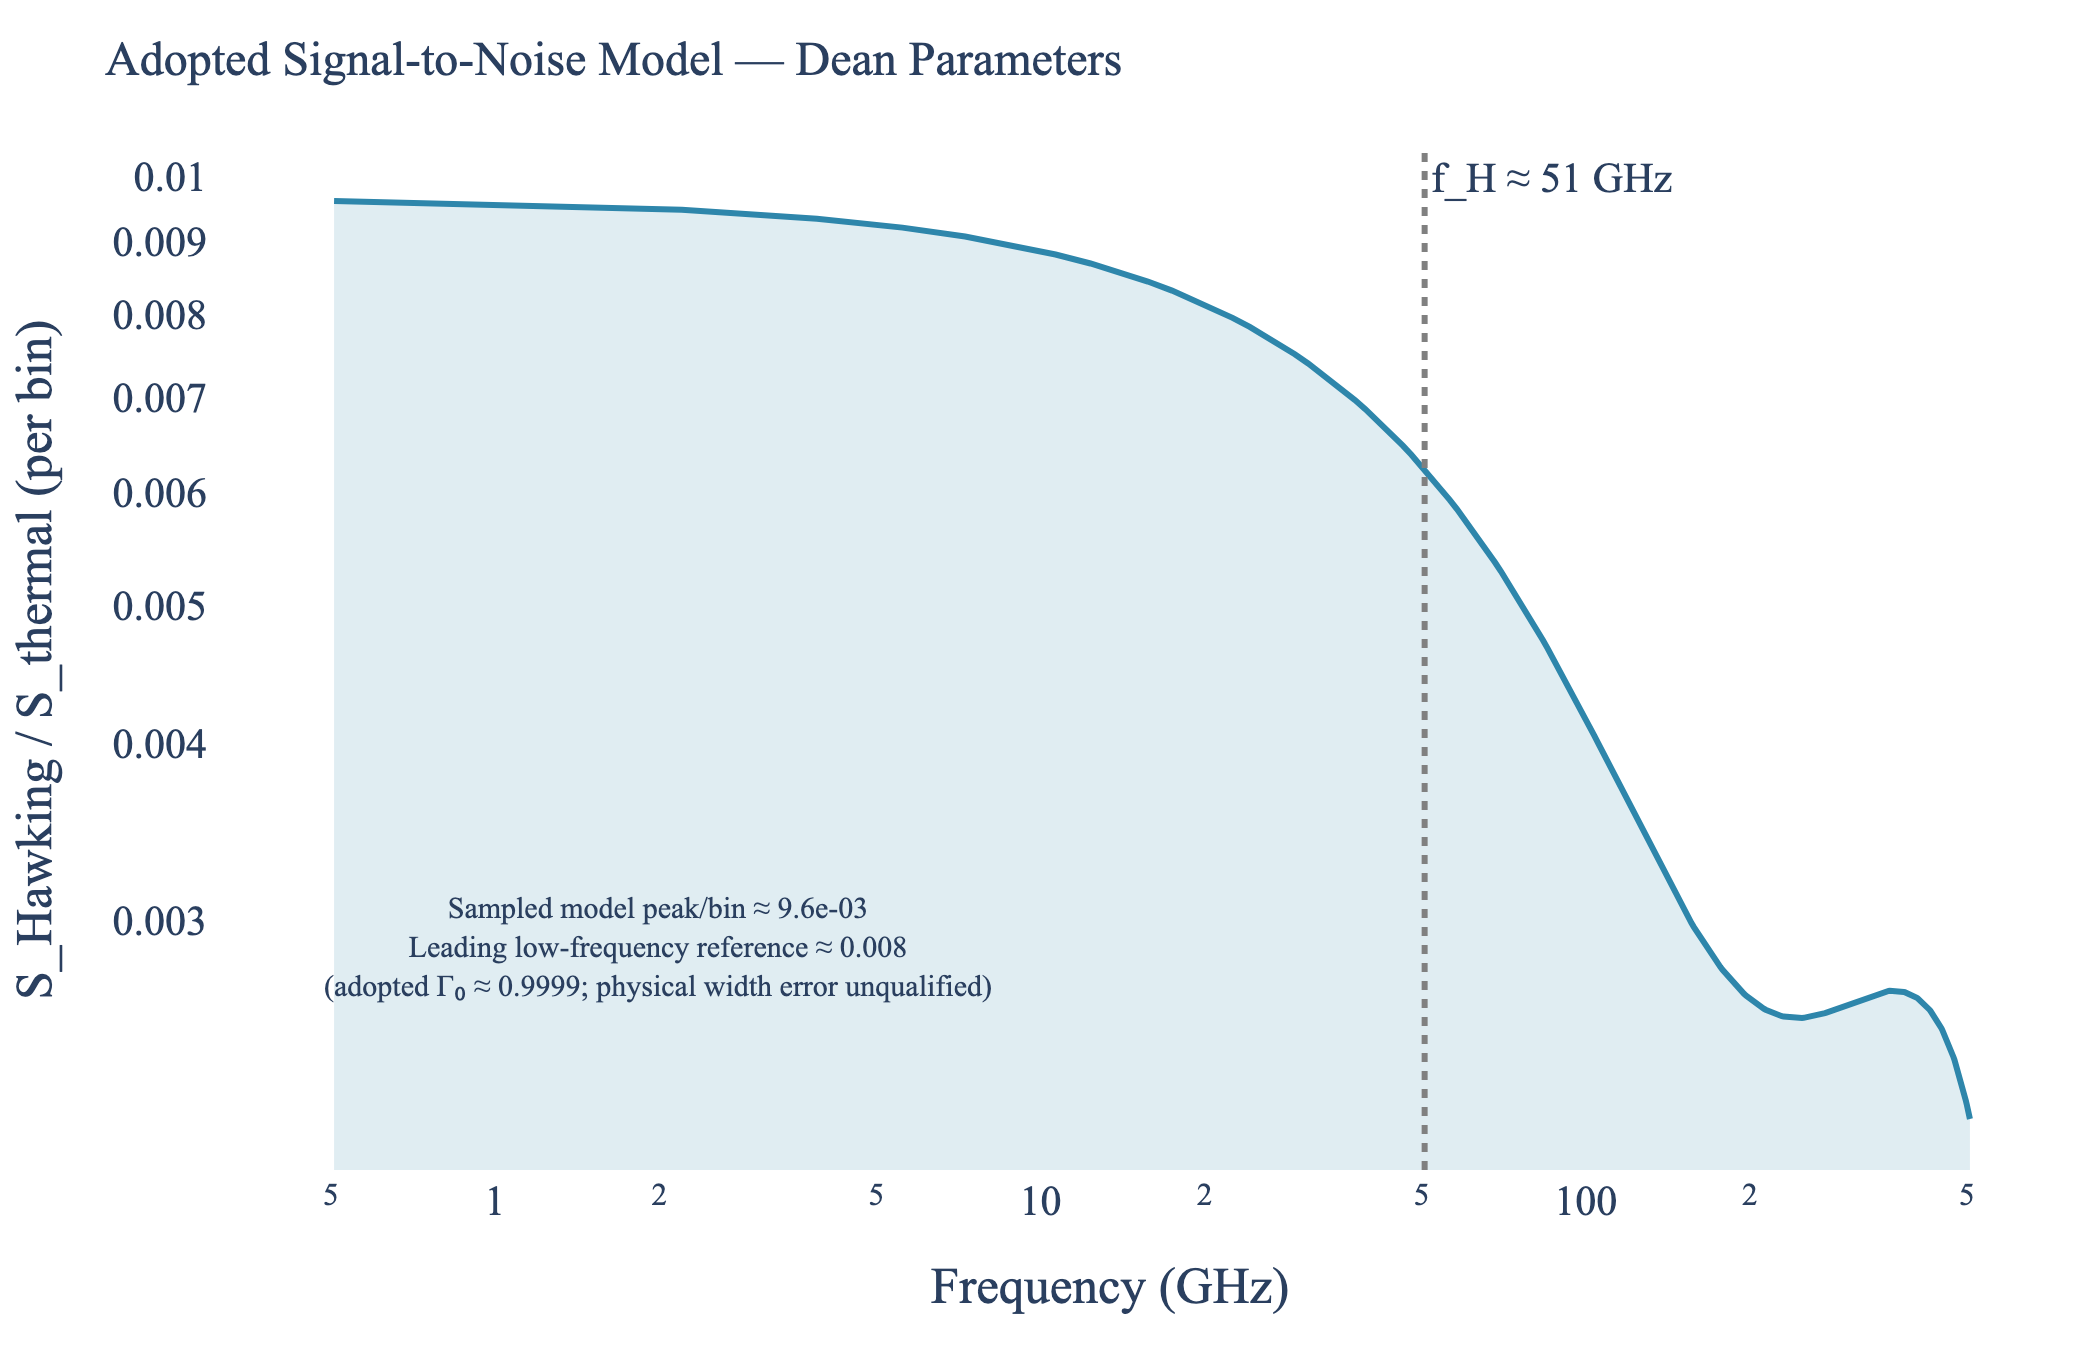
\includegraphics[width=\columnwidth]{figures/fig105_graphene_snr_frequency.png}
\caption{Adopted signal/background model at the supplied Dean inputs
$c_s=4.4\times10^5$~m/s, $\kappa=2\times10^{12}$~s$^{-1}$,
$T_H\approx2.4$~K, $\sigma_Q\approx4e^2/h$ and $T_e=150$~K.
The numerical curve includes the adopted corrected occupation/floor and
quadratic transmission. The constant-transmission leading Planck
reference tends to $\Gamma_0T_H/(2T_e)\approx8\times10^{-3}$;
that is not an exact identity for the corrected curve. The cyclic
frequency is $f_H=\omega_H/(2\pi)\approx50$~GHz.
Scalar conductance cancellation holds only within the stated common-PSD
model; physical transfer, state/noise and calibration remain required.}
\label{fig:snr}
\end{figure}

A radiometric measurement converts that fractional excess into an
integration time. For a single bin of width $\Delta f$ the standard
scaling gives $t = 1/(\mathrm{SNR}_{\rm bin}^2 \Delta f)$, so a bin of
$1$~GHz at a per-bin ratio of $8\times10^{-3}$ reaches unit
signal-to-noise in tens of microseconds, and combining the roughly $300$
independent bins across the band shortens it further. The separate shape-aware, order-of-a-minute target is not derived from
that full-grid radiometer statistic, and no calibrated estimator or
uncertainty budget for it is supplied here.
% TODO: the "of order a minute" figure is a downstream estimate from the
% shape-aware correlation analysis and is not the output of the canonical
% bandwidth-cumulative radiometer computation, which returns a far
% shorter time at the same parameters; the chain from one to the other
% is not reproduced here.
Those ideal statistics do not establish that the actual measurement is
systematics-limited or feasible. A hypothetical $\Gamma\sim10^{-2}$
and its model statistical time below a second do not determine a real
integration time. Scalar monotonicity does not establish physical
transmission, receiver efficiency or sensitivity. Independent contact,
circuit and detector noise, ordering, gain, correlations and systematic
errors are needed on the same measured band. The cited few-kelvin
amplifier illustration (roughly $2$--$5$~K against $T_e=150$~K) does not
replace actual transfer/noise calibration. Low-frequency contact noise
and non-Gaussian fluctuations can invalidate independent-bin statistics.
The transverse ratio $\omega_\perp/\omega_H\approx4.4$ is only about
$1.1$ relative to the proposed upper edge $4\omega_H$, not a factor
of $4.4$ above it. Neither this assumed channel separation nor the
supplied envelopes prove a controlled physical band.
An unknown transmission/gain/background changes shape and normalization.
Across the proposed $\omega/\omega_H\in[0.5,4]$, one uncalibrated
spectrum cannot independently identify $T_H$ and $\sigma_Q$.
After current/transfer/noise calibration and an operating-point
conductivity measurement, a fitted temperature could test a measured
sonic gradient; normalization would test the adopted response. A mismatch
while $\kappa$ is unmeasured does not by itself falsify the full framework.
The full microscopic routes, physical mode matching and identifiable
error-controlled nonempty band remain BUILD.
The device-specific version of this
prediction is developed in the companion letter~\cite{Roehm2026E2}.

\section{Exciton-polariton microcavities}
\label{sec:polariton}

The supplied condensate and Dirac-fluid inputs in
Secs.~\ref{sec:hierarchy} and~\ref{sec:graphene} satisfy the stated
scalar smallness criteria of Sec.~\ref{sec:eft}. This proves no physical convergence or
remainder bound: actual action/mode/state and observable matching remains
BUILD. The exciton-polariton inputs fail the same necessary model
criteria. Two supplied diagnostic quantities, $D$ and the decay-to-gradient
ratio, are of order unity at the measured inputs. The formal negative
statement is an inequality on these parameters, not a complete physical
theory or proof of convergence for the passing cases.

\subsection{Reservoir-corrected sound speed and the horizon}
\label{sec:pol-cs}

The reference device is the Paris-LKB polariton fluid of Falque
\emph{et al.}~\cite{Falque2025}, a semiconductor microcavity with three
InGaAs quantum wells between GaAs-AlGaAs Bragg mirrors, driven
quasi-resonantly by a continuous-wave laser whose spatial phase is
imprinted by a spatial light modulator. That imprint sets the flow
profile directly, so the horizon geometry is programmed rather than
grown. Two families of horizon were realised: smooth transitions with
surface gravity $\kappa = 0.07$ and $0.08~\mathrm{ps}^{-1}$, and a steep
configuration reaching $\kappa = 0.11~\mathrm{ps}^{-1}$. We take
$\kappa = 7\times10^{10}~\mathrm{s}^{-1}$ as the baseline and
$\kappa = 1.1\times10^{11}~\mathrm{s}^{-1}$ as the demonstrated reach.

The sound speed is the parameter that matters most for the acoustic
metric and the one most easily overestimated on this platform. Falque
\emph{et al.} determine it spectroscopically rather than
hydrodynamically. The velocity field is recovered from the spatial phase
of the outgoing light by off-axis interferometry,
$v_0(x) = \partial_x\theta$, while the Bogoliubov dispersion of the
collective excitations is measured at a chosen point by coherent probe
spectroscopy with a second continuous-wave laser, scanned in probe
wavevector and frequency, and fitted with the laboratory-frame
dispersion using the interaction energy $gn$ as the free parameter.
Because the outgoing intensity is proportional to the intracavity
density, the local sound speed follows across the whole fluid from the
measured intensity map anchored at the probed point. The result is
$c_s \approx 0.40~\mu\mathrm{m/ps}$ with an upstream healing length
$\xi \approx 3.4~\mu\mathrm{m}$ and $\xi \approx 4.0~\mu\mathrm{m}$
downstream, at an effective polariton mass
$m^* = 7.0\times10^{-35}~\mathrm{kg}$.

The reservoir correction is what separates that number from a naive
Bogoliubov estimate. Excitonic states that do not couple to light form a
long-lived dark reservoir contributing an interaction energy $g_r n_r$
to the polariton field. Falque \emph{et al.} fit their data with
$g_r n_r \approx 1.84\,gn$, so the reservoir carries roughly $65\%$ of
the total interaction blueshift. Only the condensate part enters the
dynamic response: at the turning point of the bistability loop, where
the dispersion is linear at low wavenumber, the sound speed is
$c_s = \sqrt{\hbar gn/m^*}$. A fit ignoring the reservoir would assign
the whole turning-point detuning to the condensate and would infer a
sound speed larger by $\sqrt{1+1.84} \approx 1.7$, near
$0.67~\mu\mathrm{m/ps}$. Reservoir-free modelling of polariton horizons
has used values as high as $1.0~\mu\mathrm{m/ps}$, a factor $2.5$ above
the measurement, and predictions scale steeply in $c_s$: the dispersive
parameter goes as $1/c_s$ and the noise scale as $c_s^2$.
% TODO: source not held in full text (Jacquet2022). The 1.0 um/ps
% reservoir-free value is quoted from the polariton-horizon modelling
% literature and has not been checked against that text.
Sound speeds in this range are reported for other polariton
condensates~\cite{Estrecho2021,Stepanov2019,Claude2023}.
% TODO: sources not held in full text (Estrecho2021, Stepanov2019,
% Claude2023); cited for corroboration of the measured range only.

With the surface-gravity relation of Sec.~\ref{sec:eft-metric}, the two
configurations give $T_H \approx 85~\mathrm{mK}$ and
$T_H \approx 134~\mathrm{mK}$, eight orders of magnitude above the
atomic-condensate benchmark of Sec.~\ref{sec:hierarchy}, which is the
platform's genuine advantage. One convention point must be stated
explicitly, because the primary source quotes a different figure: the
Discussion of Ref.~\cite{Falque2025} reports a Hawking temperature of
$3~\mathrm{K}$ for the smoothest horizon, which follows from the
Boltzmann exponent $\omega/2\pi\kappa$ written in their Eq.~(9) rather
than the $2\pi\omega/\kappa$ used throughout this paper. The two differ
by $4\pi^2$ at fixed $\kappa$, and the measured $\kappa$ is not in
dispute.

Two features of this platform are absent from the condensate and
graphene cases, and both weaken the horizon description. First, the
excitation field is massive. Because the fluid is driven and dissipative
rather than isolated, linearising about the steady state gives a
Klein--Gordon equation on the acoustic metric with a nonzero mass
$m_{\rm det}$ controlled by the pump detuning, not the massless equation
the isolated barotropic case delivers. A consequence is that the
acoustic horizon and the threshold for exciting negative-energy modes no
longer coincide: the Mach number that must be exceeded for a
supercritical dispersion is
$M_{\rm critical} = \sqrt{1+m_{\rm det}/m^*} = 1.34$ at the reported
parameters, not unity. Sonic-horizon formation and Hawking-type
amplification are separate conditions here, and only the second is what
an experiment sees.

Second, physical control of the adopted gradient-expansion illustration
has not been established. The dispersive parameter $D = \xi\kappa/c_s$
evaluates to $0.59$ at the smooth horizon and $0.94$ at the steep reach,
the latter using the healing length measured in the smooth configuration
because the source does not quote $\xi$ separately for the steep one.
The adopted dispersive model of Sec.~\ref{sec:eft-disp} is then $-18\%$
and $-46\%$ respectively. The smooth-horizon value is a numerical model
illustration, not a controlled physical correction: neither its size nor
$D=0.59$ supplies the missing profile/dispersion derivation or remainder
bound. The full shared physical law and error regime remain BUILD.
At the steep reach the expansion parameter is not small, the next order
is not obviously smaller than the one retained, and every steep-horizon
number in this paper is leading-order only. Buying a factor $1.6$ in
$T_H$ by steepening the horizon costs the expansion that produced the prediction.

Finally, the mean-field energy-temperature scale
$m^*c_s^2/k_B\approx0.81~\mathrm{K}$ exceeds the smooth-horizon
$T_H$ numerically. This energy comparison specifies neither a
measured noise PSD nor an occupation floor, so it cannot by itself
explain a spontaneous-detection limit or establish stimulated
detectability. The pumped state, optical/current transfer,
ordered and correlated background noise, calibration and
identifiable nonempty frequency band remain the same E1/D1 BUILD
obligations stated in the detection discussion below.

\subsection{Attenuation, and where the model provably fails}
\label{sec:pol-scope}

Cavity loss is the one dissipative channel with no counterpart in the
condensate treatment. Polaritons leak out of the cavity at a rate
$\Gamma_{\rm pol}$ set by the mirrors and independent of frequency, so
it does not enter the effective theory as a transport coefficient at
all. We treat it as a patch on the outside of the framework: the horizon
dynamics are computed as before, and the propagation of the emitted
quanta from the horizon to the detector is corrected for uniform decay.
An excitation travelling a distance $L$ at group velocity $v_g$ is
attenuated by $\exp(-\Gamma_{\rm pol}L/v_g)$, so the intrinsic
occupation is recovered from the measured one by
\begin{equation}
N_{\rm corr} = N_{\rm meas}\,
\exp\!\left(\frac{\Gamma_{\rm pol}L}{v_g}\right).
\label{eq:pol-atten}
\end{equation}

Equation~\eqref{eq:pol-atten} is
\texttt{PolaritonTier1.attenuationFactor} on the parameter record
\texttt{PolaritonParams}, which carries $\kappa > 0$,
$\Gamma_{\rm pol} \geq 0$, $v_g > 0$ and $L \geq 0$. What is formally
verified about it is exactly what an exponential gives, and we state it
as such. The exponent is non-negative
(\texttt{attenuation\_exponent\_nonneg}), so the factor is never below
unity (\texttt{attenuation\_ge\_one}): the correction can only raise an
inferred occupation, never lower it, which fixes the sign of the
systematic. It is monotone in the decay rate at fixed geometry
(\texttt{attenuation\_mono\_Gamma}), and it returns to unity when the
decay rate vanishes (\texttt{attenuation\_eq\_one\_at\_zero\_decay}),
recovering the closed-system limit. These are bookkeeping guarantees.
They are worth having because a sign-flipped or non-monotone correction
factor is a mistake that survives numerical testing, and they are not
worth more than that.

The substantive question is when the patch is legitimate at all.
Treating loss as a perturbation on the horizon dynamics requires the
decay rate to be small against the surface gravity, which is the only
inverse timescale the horizon itself supplies. The framework therefore
carries the dimensionless ratio $\Gamma_{\rm pol}/\kappa$ as
\texttt{PolaritonTier1.validityRatio}, non-negative by
\texttt{validity\_nonneg} and zero in the closed-system limit by
\texttt{validity\_zero\_at\_zero\_decay}, and the treatment is called
perturbative only below $\Gamma_{\rm pol}/\kappa = 0.1$.

Applied to the Paris-LKB device as built, that criterion is not met.
Falque \emph{et al.} measure a polariton decay rate
$\hbar\gamma \approx 80~\mu\mathrm{eV}$, that is
$\tau_{\rm cav} \approx 8~\mathrm{ps}$ and
$\Gamma_{\rm pol} \approx 1.25\times10^{11}~\mathrm{s}^{-1}$, giving
$\Gamma_{\rm pol}/\kappa \approx 1.8$ at the smooth horizon. Decay is
not a perturbation on that device; it is the fastest process at the
horizon. A cavity with $\tau_{\rm cav} = 100~\mathrm{ps}$ would give
$0.14$, still outside, and only a $300~\mathrm{ps}$ cavity brings the
ratio to $0.05$. Long-lifetime microcavities of that class exist, but
they are not the sample these horizons were made in, so every
perturbative dissipation statement in this section is a statement about
a projected device and is labelled as such in
Appendix~\ref{app:status}.

The boundary can be drawn sharply, and it is here that formalisation
pays for itself. Consider the charge-tunable MoSe$_2$ monolayer
integrated into a suspended silicon-nitride photonic-crystal nanobeam
cavity of Wang \emph{et al.}~\cite{Wang2026TMDPolariton}. That device is
not an analog-gravity experiment: it hosts no flowing condensate and
forms no sonic horizon, and its subject is nonlinear polariton response
and all-optical switching. What it supplies is a measured linewidth.
The quoted widths refer to the published 2026 report; the held author
preprint, arXiv:2411.16635v1 (2024), has a different title and author
order. We do not assume that every device parameter is identical across
these editions. In the published report's charge-neutral regime the
transmission spectrum shows upper and
lower polariton peaks with linewidths $2.3~\mathrm{meV}$ and
$\gamma_{\rm LP} = 1.8~\mathrm{meV}$, the latter corresponding to a
decoherence rate
$\Gamma_{\rm LP} = \gamma_{\rm LP}/\hbar \approx
2.73\times10^{12}~\mathrm{s}^{-1}$. Pairing that rate with the
\emph{most generous} surface gravity anywhere in the polariton family,
the steep-horizon maximum $\kappa = 1.1\times10^{11}~\mathrm{s}^{-1}$
from Ref.~\cite{Falque2025}, gives the parameter record
\texttt{PolaritonTier1.pennTmdPolaritonParams} and
\begin{equation}
\frac{\Gamma_{\rm LP}}{\kappa_{\max}} \approx 24.86 ,
\label{eq:pol-fail}
\end{equation}
roughly $250$ times the perturbative threshold. The formal statement is
\texttt{PolaritonTier1.polariton\_tier1\_fails\_tmds}, which proves
$1/10 \leq \texttt{validityRatio}$ on that record, with the companion
\texttt{polariton\_tier1\_predicate\_fails\_tmds} stating that the
perturbative predicate does not hold; both are closed by
\texttt{norm\_num} over exact rationals and introduce no assumption. Two
limitations of the encoding should be recorded. The record also carries
$v_g$ and $L$ fields, which the validity ratio does not read, and the
$v_g$ value stored there is a placeholder rather than a measured group
velocity for this device. Neither enters Eq.~\eqref{eq:pol-fail}.

What this buys is worth being explicit about, because the theorem is
trivial to prove and easy to undervalue. A narrative estimate can also
observe that ultrafast polariton linewidths are too broad for a
perturbative loss treatment. What it cannot do is bind that observation
to the same predicate that licenses the positive claims. Here the object
evaluated on the hostile input, \texttt{validityRatio}, is the object
whose smallness every perturbative dissipation statement in this section
depends on, and the failure is checked at the same threshold. A later
relaxation of the threshold to accommodate an inconvenient platform
would have to falsify a compiled theorem, and a later re-reading of
$\Gamma_{\rm pol}$ as something other than $\gamma_{\rm LP}/\hbar$ would
have to change a number that appears in the parameter provenance record.
Scope claims are the part of a theoretical framework that drifts most
quietly, because nothing downstream ever recomputes them. Compiling one
is the cheapest available way to stop that drift.

The stimulated-detection estimate that motivates the polariton platform
belongs in the same accounting, on the unverified side of it. A coherent
probe at frequency $\omega$ incident on the horizon is amplified by
anomalous Bogoliubov scattering, with emitted occupation
$G(\omega) = \Gamma(\omega)/[\exp(2\pi\omega/\kappa_{\rm eff})-1]$,
where $\Gamma(\omega)$ is the greybody factor and
$\kappa_{\rm eff} = \kappa(1+\delta_{\rm disp})$ carries the dispersive
correction of Sec.~\ref{sec:eft-disp}. Assuming unit greybody factor,
$\Gamma(\omega) = 1$, the condition $G > 1/2$ reads
$\exp(2\pi\omega/\kappa_{\rm eff}) < 3$, that is
$\omega/\kappa_{\rm eff} < \ln 3/(2\pi) \approx 0.175$. That threshold
holds only under the unit-greybody assumption stated in the same breath
as it; a dispersive horizon delivers $\Gamma(\omega) < 1$ and moves the
accessible window down. For shot-noise-limited detection of a probe
carrying $N_{\rm probe}$ photons per mode, a single-shot
signal-to-noise ratio $\sqrt{N_{\rm probe}}\,G = 5$ needs
$N_{\rm probe} = 25/G^2$, of order $10^2$ photons per mode at
$G = 1/2$, which assumes mean-field probe operation, no loss between
horizon and detector beyond Eq.~\eqref{eq:pol-atten}, and that the
background is independently calibrated and spectrally featureless across
the probe window. The quoted $0.81~\mathrm{K}$ is a mean-field energy
scale, not a measured noise PSD or occupation floor; it supplies no such
calibration. None of this paragraph is machine-checked: the formalised
polariton module contains no gain function, and the estimate is analytic
throughout.
% TODO: source not held in full text (Grisins2016), cited for the
% stimulated-detection pathway in a flowing fluid of light; the gain
% expression is stated from the framework of Sec. II, not attributed
% to that text.

These illustrations cover three platforms with distinct model-criterion
outcomes. Passing condensate and Dirac-fluid scalar inequalities leaves
physical spectrum/error and readout matching BUILD. The Paris-LKB
polariton inputs satisfy neither criterion cleanly: $D$ is of order unity
and $\Gamma_{\rm pol}/\kappa\approx1.8$. The conditional estimates in
Sec.~\ref{sec:pol-cs} require a future long-lifetime device plus actual
physical mode/state/noise reduction and calibrated readout; no such
cavity has yet been combined with a programmed horizon. Ultrafast
nanocavity inputs fail the stated scalar threshold by a factor $250$; the
checked exclusion is that model inequality.

\section{Synthesis and outlook}
\label{sec:synthesis}

The question posed in Sec.~\ref{sec:intro} was whether the analog Hawking
prediction depends on the microscopic constitution of the fluid. The
formal parameter reductions below distinguish that physical question from
identities within an adopted model; physical universality of the full
corrections remains a constructive obligation.

The leading acoustic Hawking relation is kinematic under its mode/state
and horizon hypotheses. Within the adopted effective-temperature record,
the dispersive term is the defined number $(\pi/6)D^2$ with its stated
sign; the definition has no further dispersion-shape argument.
\texttt{HawkingUniversality.hawking\_universality}
(Sec.~\ref{sec:eft-universality}) certifies that formal parameter
independence, not a derivation of a universal physical quadratic law or a
controlled profile-dependent remainder. Actual ultraviolet dispersion,
profile, state and observable matching remain the one shared BUILD.
The first-order action classification reduces nine candidate couplings
to two under its normalisation, positivity and Kubo--Martin--Schwinger
hypotheses (Sec.~\ref{sec:eft-first}); the adopted dissipative expression
uses $\gamma_1+\gamma_2$. Neither this formal reduction nor the number
of parameters supplies the complete physical horizon spectrum or its
error control for an arbitrary fluid.

The structural corroboration is the transfer to a system that shares no
microscopic physics with a condensate. Of the
\reusePopulation{} theorems in the one-dimensional inventory,
\reuseTransferred{} apply verbatim to the two-dimensional Dirac fluid
under $c_s \to v_F/\sqrt{2}$, and the ones that do not are exactly the
statements that mention the explicit $2\times2$ matrices or
condensate-specific microphysics. That is a mechanical partition rather
than an argument, and it should be read as corroboration of a claim
carried by the named theorems, not as a measurement of universality in
its own right.

The adopted numerical illustrations have different term orderings.
Table~\ref{tab:hierarchy} gives larger dispersion at $^{87}$Rb and larger
dissipation at the projected $^{39}$K and graphene inputs. The polariton
smooth-horizon entries are $-18\%$ and $+180\%$, a factor-ten disparity,
not comparable corrections. The latter uses cavity decay outside the
perturbative transport reading. These are model diagnostics, not
controlled physical orderings before law and platform matching.
In the adopted condensate spectrum, Eq.~\eqref{eq:crossover} gives
$6.44\,T_{\rm eff}$ in the one dissipation-dominated configuration.
The adopted Dirac-fluid current-noise model has conditional cancellation
of a common multiplicative conductance; actual feasibility still requires
independent current/transfer/noise and background calibration. The
polariton damping criterion supplies a separate conditional boundary:
at the supplied ultrafast nanocavity linewidths the perturbative
dissipation treatment fails by more than two orders of magnitude, and
\texttt{PolaritonTier1.polariton\_tier1\_fails\_tmds} records that inequality
against the most generous surface gravity in that stated family.

Three things follow for what a reader should do with this.

Equation~\eqref{eq:crossover} supplies a conditional shape test after
physical mode/bath/state, transmission and receiver/background responses
have been established with errors. A common amplitude may cancel; an
unknown frequency-dependent response need not. An exponential tail past
the model crossing tests that joint calibrated construction, not the
physical dissipative sector independently of its matching hypotheses.

The dependency structure separates the generic FDR relation
Eq.~\eqref{eq:cgl-fdr}, the adopted positive-scale Bogoliubov ratio,
modified unitarity Eq.~\eqref{eq:modified-unitarity}, and the separately
supplied floor/state/normalization ansatz. The first two do not by
themselves fix the floor or its physical coupling. The model crossover
requires all of these inputs plus frequency and receiver matching.
Counting, uniqueness reductions, scalar positivity and metric identities
remain at their own stated scope. Appendix~\ref{app:status} records the
distinction; completing the physical construction remains owed.

Three questions are open, and one of them is close. The strong-dissipation
regime $\Gamma_H \gtrsim \kappa$, where the perturbative connection
breaks down, is reachable in principle by complex-time methods and is
where the polariton steep-horizon configuration already sits; the
attenuation results of Sec.~\ref{sec:pol-scope} are a patch, not a
treatment. The gradient expansion assumes local dissipation, and
phonon-mediated channels in a condensate and Coulomb-mediated channels
in graphene both introduce non-local kernels whose effect on
$\delta_{\rm diss}(\omega)$ is not known. And $\gamma_1$ and
$\gamma_2$ enter as inputs: Beliaev and Landau damping supply
first-principles values for a condensate~\cite{Zaremba1999}, but the
corresponding calculations for driven-dissipative polariton kinetics and
for electron-electron scattering in a Dirac fluid are not yet at the
precision the crossover measurement would reward.

\begin{acknowledgments}
The author thanks the Aristotle team for use of the automated prover.
Its counterexample to the original first-order
Kubo--Martin--Schwinger formulation (Sec.~\ref{sec:higher-optimal}) and
its closure of the counting formula Eq.~\eqref{eq:count-formula} were
substantive contributions rather than closures of existing skeletons.
\end{acknowledgments}

\section*{Methods and tools disclosure}
The formal verification layer of this work was developed with substantial
machine assistance: Lean~4 proof drafting and iteration used LLM-based
agents (Anthropic Claude-family models) operating under the project's
staged validation pipeline. A subset of the underlying library's theorems
was closed by the Aristotle automated theorem prover (Harmonic); every
proof is ultimately certified by the Lean~4 kernel via \texttt{lake build}
on the public repository, independently of any AI tool. Manuscript prose
was AI-assisted and human-reviewed. The repository's public validation
suite reports, for every draft, any numerical value written inline in
prose rather than sourced from a generated table; that report is the
authority on this manuscript's numerical provenance.

\appendix

\section{What is and is not machine-checked}
\label{app:status}

Section~\ref{sec:intro} introduced four statuses. This appendix applies
them to every Lean result the body cites, so that a reader can see the
dependency structure without reconstructing it from the text.
\texttt{lake build} is clean over the library, with zero \texttt{sorry}
and \axiomcount{} project-local axioms beyond the three Lean~4 kernel
axioms; \aristotleproved{} of the library's theorems were closed by the
automated prover. The results reachable from this paper's claims comprise
\bundleTheorems{}~theorems across \bundleModules{}~modules.

\begin{table}[h]
\centering
\caption{Status of the Lean results cited in the body.
\emph{Derived}: the conclusion constrains something the hypotheses do not
already assert. \emph{Conditional}: the physical content is a hypothesis
and the theorem propagates it. \emph{Definitional}: the statement unfolds
a definition or rearranges a structure field. \emph{Demarcation}: a
kernel-checked statement that a model does not apply.}
\label{tab:status}
\begin{ruledtabular}
\begin{tabular}{lll}
Result & Sec. & Status \\
\colrule
\texttt{acousticMetric\_det} & \ref{sec:eft-metric} & derived \\
\texttt{acoustic\_metric\_lorentzian} & \ref{sec:eft-metric} & derived \\
\texttt{acousticMetric\_inv\_correct} & \ref{sec:eft-metric} & derived \\
\texttt{hawking\_temp\_from\_surface\_gravity} & \ref{sec:eft-metric} & definitional \\
\texttt{firstOrder\_uniqueness} & \ref{sec:eft-first} & derived \\
\texttt{deltaDissFromTransport\_eq} & \ref{sec:eft-first} & definitional \\
\texttt{deltaDissFromTransport\_zero\_iff} & \ref{sec:eft-first} & derived \\
\texttt{hawking\_universality} & \ref{sec:eft-universality} & derived \\
\texttt{transport\_coefficient\_count} & \ref{sec:higher-count} & derived \\
\texttt{firstOrder\_count}, \texttt{secondOrder\_count} & \ref{sec:higher-count} & derived \\
\texttt{thirdOrder\_count} & \ref{sec:higher-count} & derived \\
\texttt{secondOrder\_count\_with\_parity} & \ref{sec:higher-parity} & derived \\
\texttt{secondOrder\_requires\_parity\_breaking} & \ref{sec:higher-parity} & definitional \\
\texttt{fullSecondOrder\_uniqueness} & \ref{sec:higher-positivity} & derived \\
\texttt{combined\_positivity\_constraint} & \ref{sec:higher-positivity} & derived \\
\texttt{firstOrder\_KMS\_optimal} & \ref{sec:higher-optimal} & derived \\
\texttt{firstOrder\_altSign\_uniqueness\_test} & \ref{sec:higher-optimal} & derived \\
\texttt{cgl\_fdr\_general} & \ref{sec:higher-fdr} & conditional \\
\texttt{einstein\_relation} & \ref{sec:higher-fdr} & conditional \\
\texttt{cgl\_implies\_secondOrderKMS} & \ref{sec:higher-fdr} & conditional \\
\texttt{turning\_point\_shift\_pos\_iff} & \ref{sec:wkb-turning} & definitional \\
\texttt{turning\_point\_shift\_eq\_decoherence} & \ref{sec:wkb-turning} & definitional \\
\texttt{unitarity\_deficit\_eq\_decoherence} & \ref{sec:wkb-unitarity} & definitional \\
\texttt{standard\_unitarity\_recovered} & \ref{sec:wkb-unitarity} & definitional \\
\texttt{decoherence\_nonneg}, \texttt{\_zero\_iff} & \ref{sec:wkb-unitarity} & definitional \\
\texttt{noise\_floor\_eq\_delta\_diss} & \ref{sec:wkb-crossover} & definitional \\
\texttt{noise\_floor\_nonneg} & \ref{sec:wkb-crossover} & definitional \\
\texttt{occupation\_reduces\_to\_beta\_sq} & \ref{sec:wkb-crossover} & definitional \\
\texttt{total\_occupation\_nonneg} & \ref{sec:wkb-crossover} & derived \\
\texttt{noise\_dominates\_when\_beta\_small} & \ref{sec:wkb-crossover} & definitional \\
\texttt{diracFluidMetric\_gtt\_vanishes} & \ref{sec:gr-metric} & derived \\
\texttt{diracFluidMetric\_y\_offdiag\_zero} & \ref{sec:gr-metric} & definitional \\
\texttt{diracFluidMetric\_txBlock\_lorentzian\_at\_horizon} & \ref{sec:gr-metric} & derived \\
\texttt{quasi1D\_validity\_bound} & \ref{sec:gr-metric} & conditional \\
\texttt{soundSpeed\_lt\_vF} & \ref{sec:gr-subluminal} & derived \\
\texttt{hawkingNoisePSD\_greybody\_mono} & \ref{sec:gr-noise} & derived \\
\texttt{snr\_sigma\_Q\_cancels} & \ref{sec:gr-noise} & derived \\
\texttt{snr\_independent\_of\_sigma\_Q} & \ref{sec:gr-noise} & derived \\
\texttt{fdt\_consistency} & \ref{sec:gr-noise} & definitional \\
\texttt{dean\_lowest\_channel\_above\_four\_omega\_H} & \ref{sec:gr-detect} & derived \\
\texttt{attenuation\_ge\_one}, \texttt{\_mono\_Gamma} & \ref{sec:pol-scope} & derived \\
\texttt{attenuation\_eq\_one\_at\_zero\_decay} & \ref{sec:pol-scope} & definitional \\
\texttt{polariton\_tier1\_fails\_tmds} & \ref{sec:pol-scope} & demarcation \\
\end{tabular}
\end{ruledtabular}
\end{table}

Three claims in the body have no entry above because they have no formal
representative, and they are listed here rather than left to inference.
The identification of the monomial index set with the independent
transport coefficients at order $N$ (Sec.~\ref{sec:higher-count}) is an
argument of this paper. The open-system Bogoliubov relation
Eq.~\eqref{eq:modified-unitarity} with $\delta_k = 2\Gamma_H/\kappa$ is
physics input, carried in the library as a structure field
(Sec.~\ref{sec:wkb-unitarity}). The stimulated-gain threshold of
Sec.~\ref{sec:pol-scope} is an analytic estimate derived in the text and
not formalised. All three are load-bearing for at least one prediction,
and none is presented above as verified.

\begin{thebibliography}{99}

\bibitem{TindallMelloFishmanStoudenmireSels2026Science392}
J.~Tindall, A.~F.~Mello, M.~Fishman, E.~M.~Stoudenmire, D.~Sels,
\emph{Dynamics of disordered quantum systems with two- and
three-dimensional tensor networks},
Science \textbf{392}, 868 (2026),
DOI 10.1126/science.adx2728, arXiv:2503.05693.

\bibitem{Hawking1974}
S.~W.~Hawking,
\emph{Black hole explosions?},
Nature \textbf{248}, 30 (1974).

\bibitem{Unruh1981}
W.~G.~Unruh,
\emph{Experimental black-hole evaporation?},
Phys.~Rev.~Lett.~\textbf{46}, 1351 (1981).

\bibitem{Visser1998}
M.~Visser,
\emph{Acoustic black holes: horizons, ergospheres and Hawking
radiation},
Class.~Quant.~Grav.~\textbf{15}, 1767 (1998).

\bibitem{Steinhauer2016}
J.~Steinhauer,
\emph{Observation of quantum Hawking radiation and its entanglement
in an analogue black hole},
Nature Phys.~\textbf{12}, 959 (2016).

\bibitem{deNova2019}
J.~R.~M.~de~Nova \emph{et al.},
\emph{Observation of thermal Hawking radiation and its temperature
in an analogue black hole},
Nature \textbf{569}, 688 (2019).

\bibitem{Falque2025}
K.~Falque \emph{et al.},
\emph{Polariton Fluids as Quantum Field Theory Simulators on Tailored
Curved Spacetimes},
Phys.~Rev.~Lett.~\textbf{135}, 023401 (2025), arXiv:2311.01392.

\bibitem{Giacobino2025}
E.~Giacobino, M.~J.~Jacquet,
\emph{Acoustic horizons and the Hawking effect in polariton
fluids of light},
arXiv:2512.14194 (2025).

\bibitem{Geurs2025}
J.~Geurs \emph{et al.},
\emph{Supersonic flow and hydraulic jump in an electronic de Laval
nozzle},
arXiv:2509.16321 (2025).

\bibitem{Majumdar2025}
A.~Majumdar \emph{et al.},
\emph{Universality in quantum critical flow of charge and heat in
ultra-clean graphene},
Nature Physics \textbf{21}, 1374 (2025), arXiv:2501.03193.

\bibitem{CGL2017a}
M.~Crossley, P.~Glorioso, and H.~Liu,
\emph{Effective field theory of dissipative fluids} (paper~I),
JHEP \textbf{09}, 095 (2017), arXiv:1511.03646.

\bibitem{GloriosoLiu2018}
P.~Glorioso and H.~Liu,
\emph{The second law of thermodynamics from symmetry and unitarity},
arXiv:1612.07705 (2016).

\bibitem{Crossley2017II}
P.~Glorioso, M.~Crossley, and H.~Liu,
\emph{Effective field theory of dissipative fluids (II):
classical limit, dynamical KMS symmetry and entropy current},
JHEP \textbf{09}, 096 (2017).

\bibitem{Jana2020}
C.~Jana, R.~Loganayagam, M.~Rangamani,
\emph{Open quantum systems and Schwinger-Keldysh holograms},
JHEP \textbf{07}, 242 (2020),
arXiv:2004.02888.

\bibitem{Son2002}
D.~T.~Son,
\emph{Low-Energy Quantum Effective Action for Relativistic
Superfluids},
arXiv:hep-ph/0204199 (2002).

\bibitem{Zaremba1999}
E.~Zaremba, T.~Nikuni, and A.~Griffin,
\emph{Dynamics of trapped Bose gases at finite temperatures},
J.~Low Temp.~Phys.~\textbf{116}, 277 (1999).

\bibitem{Berry1989}
M.~V.~Berry,
\emph{Uniform asymptotic smoothing of Stokes's discontinuities},
Proc.~R.~Soc.~Lond.~A \textbf{422}, 7 (1989).

\bibitem{Heading1962}
J.~Heading,
\emph{An Introduction to Phase-Integral Methods},
Methuen, London (1962).

\bibitem{CorleyJacobson1996}
S.~Corley and T.~Jacobson,
\emph{Hawking spectrum and high-frequency dispersion},
Phys.~Rev.~D \textbf{54}, 1568 (1996).

\bibitem{Coutant2014}
A.~Coutant and R.~Parentani,
\emph{Hawking radiation with dispersion: the broadened horizon paradigm},
Phys.~Rev.~D \textbf{90}, 121501(R) (2014), arXiv:1402.2514.

\bibitem{CoutantParentani2012}
A.~Coutant, R.~Parentani, S.~Finazzi,
\emph{Black hole radiation with short distance dispersion, an
analytical S-matrix approach},
Phys.~Rev.~D \textbf{85}, 024021 (2012).

\bibitem{RobertsonParentani2015}
S.~Robertson, R.~Parentani,
\emph{Hawking radiation in the presence of high-momentum
dissipation},
Phys.~Rev.~D \textbf{92}, 044043 (2015).

\bibitem{BelgiornoCacciatori2024}
F.~Belgiorno, S.~L.~Cacciatori, S.~Trevisan,
\emph{Analogous Hawking Radiation in Dispersive Media},
Universe~\textbf{10}, 412 (2024). DOI: \href{https://doi.org/10.3390/universe10110412}{10.3390/universe10110412}.

\bibitem{Viermann2022}
C.~Viermann \emph{et al.},
\emph{Quantum field simulator for dynamics in curved spacetime},
Nature \textbf{611}, 260 (2022). DOI: \href{https://doi.org/10.1038/s41586-022-05313-9}{10.1038/s41586-022-05313-9}.

\bibitem{Estrecho2021}
E.~Estrecho \emph{et al.},
\emph{Low-energy collective oscillations and Bogoliubov sound
in an exciton-polariton condensate},
Phys.~Rev.~Lett.~\textbf{126}, 075301 (2021).

\bibitem{Stepanov2019}
P.~Stepanov \emph{et al.},
\emph{Dispersion relation of the collective excitations in a
resonantly driven polariton fluid},
Nature Comm.~\textbf{10}, 3869 (2019).

\bibitem{Claude2023}
F.~Claude \emph{et al.},
\emph{Spectrum of collective excitations of a quantum fluid of polaritons},
Phys.~Rev.~B~\textbf{107}, 174507 (2023).

\bibitem{Grisins2016}
P.~Gri\v{s}ins, H.~S.~Nguyen, J.~Bloch, A.~Amo, I.~Carusotto,
\emph{Theoretical study of stimulated and spontaneous Hawking
effects from an acoustic black hole in a hydrodynamically flowing
fluid of light},
Phys.~Rev.~B \textbf{94}, 144518 (2016).

\bibitem{Burkhard2025}
M.~Burkhard \emph{et al.},
\emph{Stimulated Hawking effect and quasinormal mode resonance in a
polariton simulator of field theory on curved spacetime},
arXiv:2511.12339 (2025).

\bibitem{Jacquet2022}
M.~Jacquet \emph{et al.},
\emph{Analogue quantum simulation of the Hawking effect in a
polariton superfluid},
Eur.~Phys.~J.~D \textbf{76}, 152 (2022).

\bibitem{Jacquet2023QNM}
M.~J.~Jacquet \emph{et al.},
\emph{Quantum Vacuum Excitation of a Quasinormal Mode in an
Analog Model of Black Hole Spacetime},
Phys.~Rev.~Lett.~\textbf{130}, 111501 (2023).

\bibitem{Zhao2023}
W.~Zhao \emph{et al.},
\emph{Observation of hydrodynamic plasmons and energy waves in
graphene},
Nature \textbf{614}, 688 (2023).

\bibitem{AndersonBFP2014Graybody}
P.~R.~Anderson, R.~Balbinot, A.~Fabbri, and R.~Parentani,
\emph{Gray-body factor and infrared divergences in 1D BEC acoustic black holes},
Phys.~Rev.~D \textbf{90}, 104044 (2014), arXiv:1404.3224v3.

\bibitem{Roehm2026Wave1}
J.~Roehm, in preparation (2026), Phase 5d wave (BEC SK-EFT first
order).

\bibitem{Roehm2026Wave2}
J.~Roehm, in preparation (2026), Phase 5d wave (BEC SK-EFT second
order).

\bibitem{Roehm2026Wave4}
J.~Roehm, in preparation (2026), Phase 5d wave (exact WKB
connection).

\bibitem{Roehm2026Wave12}
J.~Roehm, in preparation (2026), Phase 5u wave (polariton
predictions).

\bibitem{Roehm2026Wave16}
J.~Roehm, in preparation (2026), Phase 5w wave (graphene Dirac-fluid
predictions).

\bibitem{Roehm2026E1}
J.~Roehm, ``A Falsifiable Hawking Spectrum for Polariton
Microcavities at the Paris LKB Device Parameters'', PRL/PRR letter
(2026).

\bibitem{Roehm2026E2}
J.~Roehm, ``Detecting Analog Hawking Radiation in the
Bilayer-Graphene Dirac Fluid'', PRL/PRR letter (2026).

\bibitem{Roehm2026F}
J.~Roehm, ``Fluid-Based Approaches to Fundamental Physics: A
Formally Verified Survey'', RMP/Phys.~Rep.~flagship review (2026).

\bibitem{Roehm2026I1}
J.~Roehm, ``Formal Verification at Scale in Theoretical Physics:
A Methodology with Worked Cases'', CPC methodology paper (2026).

\bibitem{Roehm2026I2}
J.~Roehm, ``Verified Statistical Estimators and the
\texttt{lean-tensor-categories} Library'', JOSS software paper (2026).



\bibitem{Wang2026TMDPolariton}
Z.~Wang, B.~Kim, B.~Zhen, and L.~He,
\emph{Strongly Nonlinear Nanocavity Exciton Polaritons in Gate-Tunable
Monolayer Semiconductors},
Phys.~Rev.~Lett.~\textbf{136}, 146901 (2026),
DOI:10.1103/gc15-qsvf; author preprint arXiv:2411.16635.

\end{thebibliography}

\end{document}
